\PassOptionsToPackage{unicode=true}{hyperref} % options for packages loaded elsewhere
\PassOptionsToPackage{hyphens}{url}
%
\documentclass[]{book}
\usepackage{lmodern}
\usepackage{amssymb,amsmath}
\usepackage{ifxetex,ifluatex}
\usepackage{fixltx2e} % provides \textsubscript
\ifnum 0\ifxetex 1\fi\ifluatex 1\fi=0 % if pdftex
  \usepackage[T1]{fontenc}
  \usepackage[utf8]{inputenc}
  \usepackage{textcomp} % provides euro and other symbols
\else % if luatex or xelatex
  \usepackage{unicode-math}
  \defaultfontfeatures{Ligatures=TeX,Scale=MatchLowercase}
\fi
% use upquote if available, for straight quotes in verbatim environments
\IfFileExists{upquote.sty}{\usepackage{upquote}}{}
% use microtype if available
\IfFileExists{microtype.sty}{%
\usepackage[]{microtype}
\UseMicrotypeSet[protrusion]{basicmath} % disable protrusion for tt fonts
}{}
\IfFileExists{parskip.sty}{%
\usepackage{parskip}
}{% else
\setlength{\parindent}{0pt}
\setlength{\parskip}{6pt plus 2pt minus 1pt}
}
\usepackage{hyperref}
\hypersetup{
            pdftitle={Climate models for ecologist},
            pdfauthor={Isaac Brito-Morales},
            pdfborder={0 0 0},
            breaklinks=true}
\urlstyle{same}  % don't use monospace font for urls
\usepackage[left=2.54cm, right=2.54cm, top=2.54cm, bottom=2.54cm]{geometry}
\usepackage{color}
\usepackage{fancyvrb}
\newcommand{\VerbBar}{|}
\newcommand{\VERB}{\Verb[commandchars=\\\{\}]}
\DefineVerbatimEnvironment{Highlighting}{Verbatim}{commandchars=\\\{\}}
% Add ',fontsize=\small' for more characters per line
\usepackage{framed}
\definecolor{shadecolor}{RGB}{248,248,248}
\newenvironment{Shaded}{\begin{snugshade}}{\end{snugshade}}
\newcommand{\AlertTok}[1]{\textcolor[rgb]{0.94,0.16,0.16}{#1}}
\newcommand{\AnnotationTok}[1]{\textcolor[rgb]{0.56,0.35,0.01}{\textbf{\textit{#1}}}}
\newcommand{\AttributeTok}[1]{\textcolor[rgb]{0.77,0.63,0.00}{#1}}
\newcommand{\BaseNTok}[1]{\textcolor[rgb]{0.00,0.00,0.81}{#1}}
\newcommand{\BuiltInTok}[1]{#1}
\newcommand{\CharTok}[1]{\textcolor[rgb]{0.31,0.60,0.02}{#1}}
\newcommand{\CommentTok}[1]{\textcolor[rgb]{0.56,0.35,0.01}{\textit{#1}}}
\newcommand{\CommentVarTok}[1]{\textcolor[rgb]{0.56,0.35,0.01}{\textbf{\textit{#1}}}}
\newcommand{\ConstantTok}[1]{\textcolor[rgb]{0.00,0.00,0.00}{#1}}
\newcommand{\ControlFlowTok}[1]{\textcolor[rgb]{0.13,0.29,0.53}{\textbf{#1}}}
\newcommand{\DataTypeTok}[1]{\textcolor[rgb]{0.13,0.29,0.53}{#1}}
\newcommand{\DecValTok}[1]{\textcolor[rgb]{0.00,0.00,0.81}{#1}}
\newcommand{\DocumentationTok}[1]{\textcolor[rgb]{0.56,0.35,0.01}{\textbf{\textit{#1}}}}
\newcommand{\ErrorTok}[1]{\textcolor[rgb]{0.64,0.00,0.00}{\textbf{#1}}}
\newcommand{\ExtensionTok}[1]{#1}
\newcommand{\FloatTok}[1]{\textcolor[rgb]{0.00,0.00,0.81}{#1}}
\newcommand{\FunctionTok}[1]{\textcolor[rgb]{0.00,0.00,0.00}{#1}}
\newcommand{\ImportTok}[1]{#1}
\newcommand{\InformationTok}[1]{\textcolor[rgb]{0.56,0.35,0.01}{\textbf{\textit{#1}}}}
\newcommand{\KeywordTok}[1]{\textcolor[rgb]{0.13,0.29,0.53}{\textbf{#1}}}
\newcommand{\NormalTok}[1]{#1}
\newcommand{\OperatorTok}[1]{\textcolor[rgb]{0.81,0.36,0.00}{\textbf{#1}}}
\newcommand{\OtherTok}[1]{\textcolor[rgb]{0.56,0.35,0.01}{#1}}
\newcommand{\PreprocessorTok}[1]{\textcolor[rgb]{0.56,0.35,0.01}{\textit{#1}}}
\newcommand{\RegionMarkerTok}[1]{#1}
\newcommand{\SpecialCharTok}[1]{\textcolor[rgb]{0.00,0.00,0.00}{#1}}
\newcommand{\SpecialStringTok}[1]{\textcolor[rgb]{0.31,0.60,0.02}{#1}}
\newcommand{\StringTok}[1]{\textcolor[rgb]{0.31,0.60,0.02}{#1}}
\newcommand{\VariableTok}[1]{\textcolor[rgb]{0.00,0.00,0.00}{#1}}
\newcommand{\VerbatimStringTok}[1]{\textcolor[rgb]{0.31,0.60,0.02}{#1}}
\newcommand{\WarningTok}[1]{\textcolor[rgb]{0.56,0.35,0.01}{\textbf{\textit{#1}}}}
\usepackage{longtable,booktabs}
% Fix footnotes in tables (requires footnote package)
\IfFileExists{footnote.sty}{\usepackage{footnote}\makesavenoteenv{longtable}}{}
\usepackage{graphicx,grffile}
\makeatletter
\def\maxwidth{\ifdim\Gin@nat@width>\linewidth\linewidth\else\Gin@nat@width\fi}
\def\maxheight{\ifdim\Gin@nat@height>\textheight\textheight\else\Gin@nat@height\fi}
\makeatother
% Scale images if necessary, so that they will not overflow the page
% margins by default, and it is still possible to overwrite the defaults
% using explicit options in \includegraphics[width, height, ...]{}
\setkeys{Gin}{width=\maxwidth,height=\maxheight,keepaspectratio}
\setlength{\emergencystretch}{3em}  % prevent overfull lines
\providecommand{\tightlist}{%
  \setlength{\itemsep}{0pt}\setlength{\parskip}{0pt}}
\setcounter{secnumdepth}{5}
% Redefines (sub)paragraphs to behave more like sections
\ifx\paragraph\undefined\else
\let\oldparagraph\paragraph
\renewcommand{\paragraph}[1]{\oldparagraph{#1}\mbox{}}
\fi
\ifx\subparagraph\undefined\else
\let\oldsubparagraph\subparagraph
\renewcommand{\subparagraph}[1]{\oldsubparagraph{#1}\mbox{}}
\fi

% set default figure placement to htbp
\makeatletter
\def\fps@figure{htbp}
\makeatother

\usepackage{booktabs}
\usepackage[]{natbib}
\bibliographystyle{apalike}

\title{Climate models for ecologist}
\author{Isaac Brito-Morales}
\date{2021-09-02}

\begin{document}
\maketitle

{
\setcounter{tocdepth}{1}
\tableofcontents
}
\hypertarget{welcome}{%
\chapter{Welcome}\label{welcome}}

This document has for objective explain how to process and calculate climate change models to estimate climate change metrics.

\hypertarget{cmip6-models}{%
\chapter{CMIP6 models}\label{cmip6-models}}

\textbf{CMIP6} stands for Coupled Model Intercomparison Project (CMIP). These are climate models that simulate the physics, chemistry and biology of the atmosphere in detail (some of them!). The 2013 IPCC fifth assessment report (AR5) featured climate models from CMIP5, while the upcoming 2021 IPCC sixth assessment report (AR6) will feature new state-of-the-art CMIP6 models (\href{https://www.carbonbrief.org/cmip6-the-next-generation-of-climate-models-explained}{more info in Carbon Brief website.})

The main goal is to set future climate scenarios based on \emph{future} concentrations of \textbf{greenhouse gases}, \textbf{aerosols} and other \href{https://www.carbonbrief.org/qa-how-do-climate-models-work\#inout}{\textbf{climate forcings}} to project what might happen in the future.

\begin{center}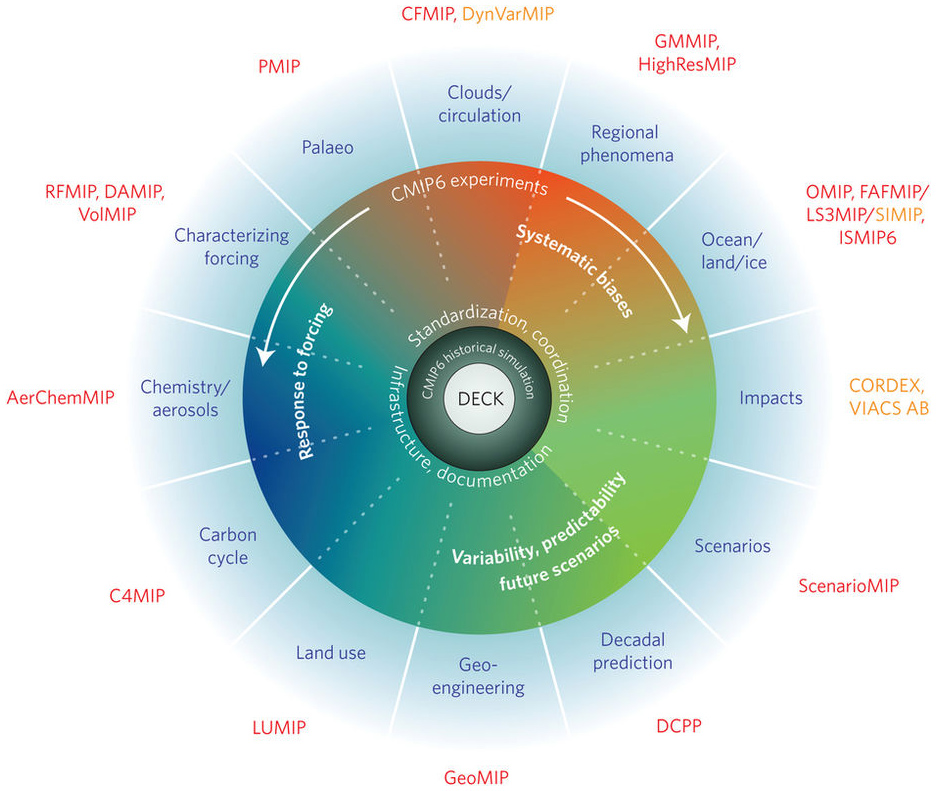
\includegraphics[width=1\linewidth]{images/cmip6_mips} \end{center}

Schematic of the CMIP/CMIP6 experimental design

\hypertarget{most-common-climate-scenarios}{%
\section{Most common climate scenarios}\label{most-common-climate-scenarios}}

From CMIP5 version you will find those as RCPs (Representative Concentration Pathways) but for the new CMIP6 version they are called SSPs (Shared Socio‐Economic Pathways).

\begin{center}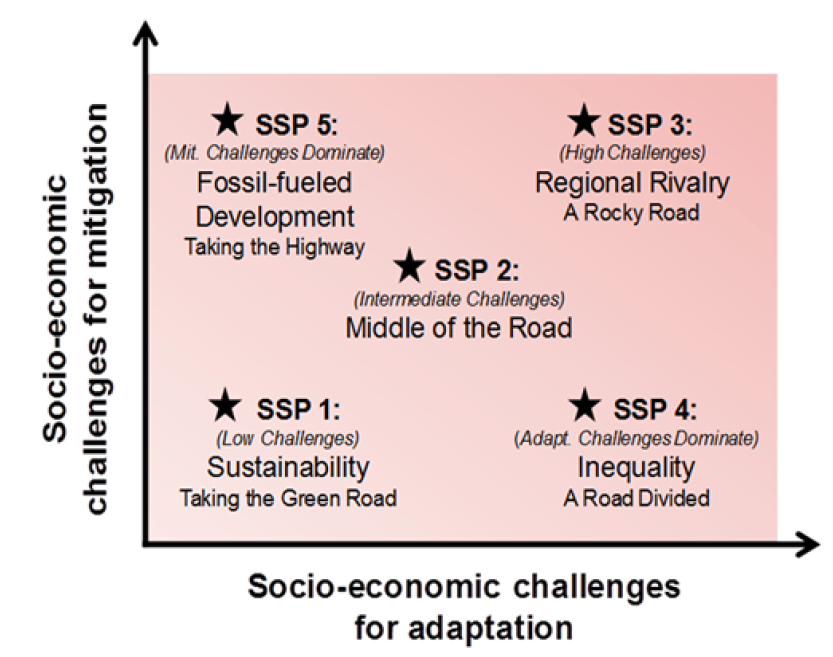
\includegraphics[width=1\linewidth]{images/ssps} \end{center}

Overview of SSPs

\textbf{Most commonly SSPs used}:

\begin{itemize}
\tightlist
\item
  SSP1-2.6: An optimistic scenario, characterised by a shift to a more sustainable economy and reduction in inequality resulting in a peak in radiative forcing of \textasciitilde{}3 W m-2 before 2100
\item
  SSP2-4.5: An intermediate scenario, with a stabilisation of radiative forcing levels at \textasciitilde{}4.5 W m-2 by 2100
\item
  SSP5-8.5: Characterised by a continued increase of greenhouse gas emissions resulting from a fossil-fuel-based economy and increased energy demand, with a radiative forcing \textgreater{}8.5 W m-2 by 2100
\end{itemize}

\hypertarget{how-to-download-cmip6-models}{%
\section{How to download CMIP6 models}\label{how-to-download-cmip6-models}}

CMIP6 models are free available at the \href{https://esgf.llnl.gov/}{\textbf{Earth System Grid Federation}} website. You will need an account to download models. \href{https://esgf.github.io/esgf-user-support/user_guide.html}{\textbf{Check this tutorial}} of how to create an account.

Through the website:

\begin{itemize}
\tightlist
\item
  Click \href{https://esgf.llnl.gov/}{here} to open the ESGF website
\item
  Go to the \emph{Nodes} tab to explore the different ESGF-CoG nodes
\item
  Click the \href{https://esgf.nci.org.au/projects/esgf-nci/}{NCI} link, the Australia National Computational Infrastructure node
\end{itemize}

Select a \href{https://esgf.nci.org.au/projects/esgf-nci/}{NCI} node, go to collection and then \href{https://esgf.nci.org.au/search/cmip6-nci/}{CMIP6} link. This is the main website to download CMIP6 models. At your left you have several filters that you can play with, my advice is filter first for variable.

\hypertarget{variables}{%
\subsection{Variables}\label{variables}}

There are a range of variables available from the GCM (General Circulation Model) outputs. Each tab has different model variable on different time scales. The tabs are in alphabetical order. The ones starting with ``O'' are for Ocean, and then followed by the timescale (clim = climatology, day, dec = decade, mon = month, yr) (source: \href{https://mathmarecol.github.io/Welcome/}{Mathematical Marine Ecology Welcome Book Chapter 9}).

From the left tab:

\begin{itemize}
\tightlist
\item
  click the \textbf{+} in the \textbf{variable} option. Select \textbf{tos} (ocean temperature on surface). Then click \textbf{Search}
\item
  click the \textbf{+} in the \textbf{Realm} option. Select \textbf{ocean} and \textbf{ocnBgChem}. Then click \textbf{Search}
\item
  click the \textbf{+} in the \textbf{Frequency} option. Select \textbf{mon}. Then click \textbf{Search}
\item
  click the \textbf{+} in the \textbf{Variant Label} option. Select \textbf{r1i1p1f1} (this is the most common ensemble). Then click \textbf{Search}
\end{itemize}

The ensemble names ``r1i1p1'', ``r2i1p1'', etc. in \textbf{Variant Label} indicate that the ensemble members differ only in their initial conditions (the model physics are the same for all ensemble members, but the members were initialized from different initial conditions out of the control simulation). Hence, the differences between the ensemble members represent internal variability.

\begin{itemize}
\tightlist
\item
  click the \textbf{+} in the \textbf{Experiment ID} option. In this option you will see every single \emph{Experiment/Simulation}. For example, \textbf{G1/G6/G7} are the geoengineering climate scenarios. Go to the bottom of the \textbf{Experiment ID} tab and click \textbf{ssp126}. Then click \textbf{Search}
\item
  click the \textbf{+} in the \textbf{Source ID} option for the full model list and their Institution ID. Let's click on \textbf{ACCESS-CM2} model from the CSIRO. Then click \textbf{Search}
\end{itemize}

If you have follow the previous steps you should get a tab result similar to this:

\begin{center}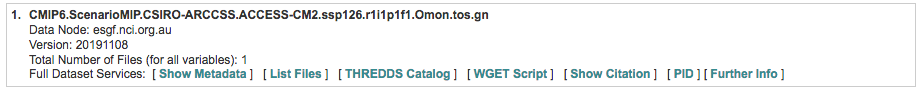
\includegraphics[width=1\linewidth]{images/model_example_tab} \end{center}

To download the model, just click on the \textbf{List Files} tab and then select \textbf{HTTP Download}

\hypertarget{getting-started-with-climate-data-operators-cdo}{%
\chapter{Getting Started with Climate Data Operators (CDO)}\label{getting-started-with-climate-data-operators-cdo}}

\textbf{CMIP6} models come in netCDF file format and they are usually really messy to work in R. For example, the resolution of the \textbf{CMIP6} NOAA model (SSP1-2.6) is 0.25°. Let say that you want to download that model for the \textbf{thetao} variable (sea temperature with depth). The size of that model is \textasciitilde{}80gb. It will be really hard just to read that file in R.

The intention with this information and scripts is to provide a basic understanding of how you can use \textbf{CDO} to speed-up your \textbf{netCDF} file data manipulation. \href{https://code.mpimet.mpg.de/projects/cdo/}{More info go directly to the Max Planck Institute CDO website}

\hypertarget{installation-process}{%
\section{Installation Process}\label{installation-process}}

\hypertarget{macos}{%
\subsection{\texorpdfstring{\textbf{MacOS}}{MacOS}}\label{macos}}

Follow the instruction and downloaded \textbf{MacPorts}. \textbf{MacPorts} is an open-source community initiative to design an easy-to-use system for compiling, installing, and upgrading the command-line on the Mac operating system.

\href{https://www.macports.org/index.php}{MacPorts website}
\href{https://www.macports.org/install.php}{MacPorts download}

After the installation (if you have admin rights) open the terminal and type:

\texttt{port\ install\ cdo}

If you don't have admin rights, open the terminal and type:

\texttt{sudo\ port\ install\ cdo} and write your password

\hypertarget{windows-10}{%
\subsection{\texorpdfstring{\textbf{Windows 10}}{Windows 10}}\label{windows-10}}

In the current windows 10 version(s) Microsoft includes an Ubuntu 16.04 LTS embedded Linux. This environment offers a clean integration with the windows file systems and and the opportunity to install CDO via the native package manager of Ubuntu.

Install the Ubuntu app from the Microsoft Store application. Then open the Ubuntu terminal and type:

\texttt{sudo\ apt-get\ install\ cdo} and write your password

\hypertarget{linux}{%
\section{\texorpdfstring{\textbf{Linux}}{Linux}}\label{linux}}

For Linux go to: \href{https://code.mpimet.mpg.de/projects/cdo/wiki/Linux_Platform}{Linux}

\hypertarget{ncview-a-netcdf-visual-browser}{%
\section{Ncview: a netCDF visual browser}\label{ncview-a-netcdf-visual-browser}}

Ncview is quick visual browser that allows you to explore \textbf{netCDF} files very easily: \texttt{ncview}. \texttt{ncview} is an easy to use netCDF file viewer for \textbf{linux} and \textbf{OS X}. It can read any netCDF file.

To install \textbf{ncview}, open the terminal and type:

\begin{itemize}
\tightlist
\item
  \textbf{OS X}: \texttt{port\ install\ ncview}
\item
  \textbf{Linux}: \texttt{sudo\ apt-get\ install\ ncview}
\end{itemize}

\hypertarget{working-with-cdo}{%
\section{Working with CDO}\label{working-with-cdo}}

To work with \textbf{CDO} and \textbf{ncview} we need to use the terminal command line: the \textbf{Ubuntu app} in Windows and the \textbf{Terminal} on OS X.

\begin{Shaded}
\begin{Highlighting}[]
\CommentTok{# Establish the primary directory (OS or Linux)}
\CommentTok{## cd ~/data/ClimateModels/tos/ssp585/}

\CommentTok{# Establish the primary directory in Windows. It should be located at "/mnt/c/"}
\CommentTok{## cd ~/data/ClimateModels/tos/ssp585/}

\CommentTok{# View the model with ncview}
\CommentTok{## ncview tos_Omon_GFDL-CM4_ssp585_r1i1p1f1_gr_201501-203412.nc}
\end{Highlighting}
\end{Shaded}

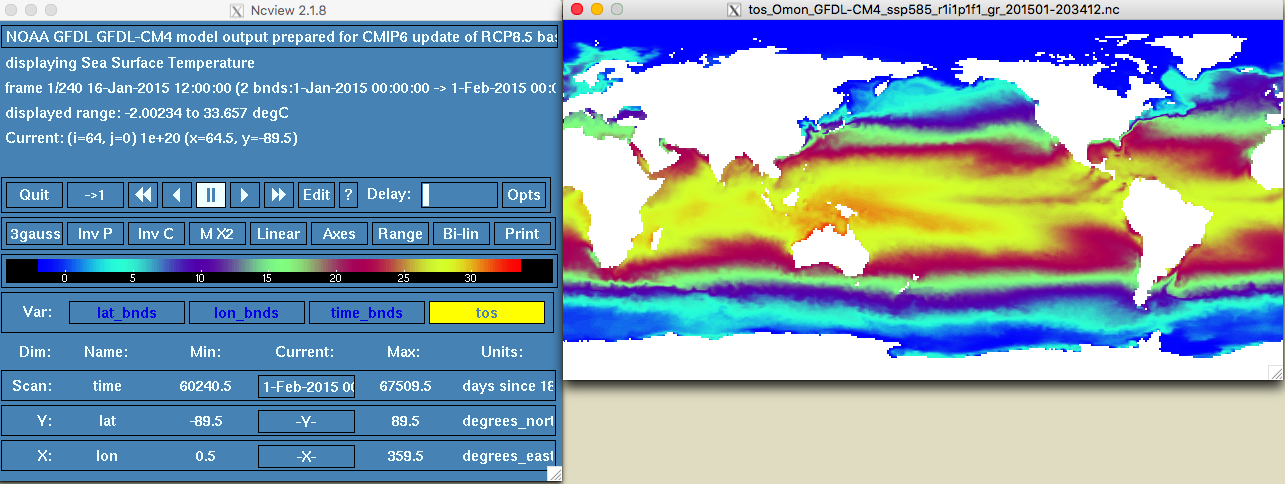
\includegraphics[width=1\linewidth]{images/ncview01}

ncview example

\begin{Shaded}
\begin{Highlighting}[]
\CommentTok{# Check the details by typing in the terminal}
\CommentTok{## cdo -sinfov tos_Omon_GFDL-CM4_ssp585_r1i1p1f1_gr_201501-203412.nc}
\end{Highlighting}
\end{Shaded}

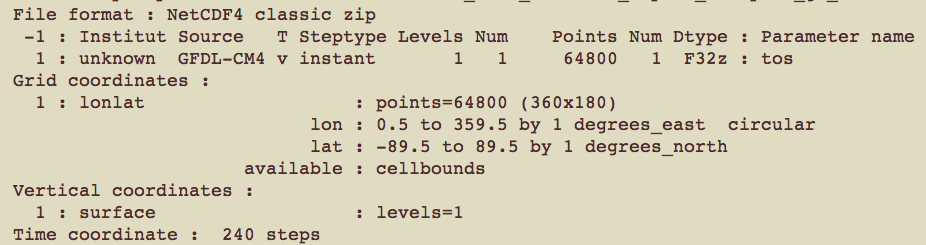
\includegraphics[width=1\linewidth]{images/ncview02}

Model details

\hypertarget{regrid-process}{%
\subsection{Regrid process}\label{regrid-process}}

To regrid a \textbf{netCDF} file using \textbf{CDO} we need to use the argument \texttt{remapbil}, which is the stands for bilinear interpolation (there are other methods but this is the most conservative approach). CDO Syntax works like this:

\begin{Shaded}
\begin{Highlighting}[]
\CommentTok{# Type in the terminal}
\CommentTok{## cdo remapbil,r360x180 tos_Omon_GFDL-CM4_ssp585_r1i1p1f1_gr_201501-203412.nc test.nc}
\end{Highlighting}
\end{Shaded}

The previous line will create an uniform file at 1deg of spatial resolution. It works fine for one or two \textbf{netCDF} files. However, for multiple \textbf{netCDF} files/models (which is most cases of CMIP6 models) the best way to auto the process is to write an \emph{R} script that calls CDO through the \textbf{system()} function.

This function will help to search for ANY \textbf{netCDF} file in a particular directory and do the ``regridding process''.

\begin{itemize}
\tightlist
\item
  \textbf{Key CDO function}: \texttt{remapbil}
\end{itemize}

\begin{Shaded}
\begin{Highlighting}[]

\CommentTok{# This code was written by Isaac Brito-Morales (i.britomorales@uq.edu.au)}
\CommentTok{# Please do not distribute this code without permission.}
\CommentTok{# NO GUARANTEES THAT CODE IS CORRECT}
\CommentTok{# Caveat Emptor!}

\CommentTok{# Function's arguments}
\CommentTok{# ipath: directory where the netCDF files are located}
\CommentTok{# opath: directory to allocate the new regrided netCDF files}
\CommentTok{# resolution = resolution for the regrid process}

\NormalTok{regrid <-}\StringTok{ }\ControlFlowTok{function}\NormalTok{(ipath, opath, resolution) \{}

\CommentTok{####################################################################################}
\CommentTok{####### Defining the main packages}
\CommentTok{####################################################################################}
  \CommentTok{# List of pacakges that we will be used}
\NormalTok{    list.of.packages <-}\StringTok{ }\KeywordTok{c}\NormalTok{(}\StringTok{"doParallel"}\NormalTok{, }\StringTok{"parallel"}\NormalTok{, }\StringTok{"stringr"}\NormalTok{, }\StringTok{"data.table"}\NormalTok{)}
  \CommentTok{# If is not installed, install the pacakge}
\NormalTok{    new.packages <-}\StringTok{ }\NormalTok{list.of.packages[}\OperatorTok{!}\NormalTok{(list.of.packages }\OperatorTok\StringTok{ }\KeywordTok{installed.packages}\NormalTok{()[,}\StringTok{"Package"}\NormalTok{])]}
    \ControlFlowTok{if}\NormalTok{(}\KeywordTok{length}\NormalTok{(new.packages)) }\KeywordTok{install.packages}\NormalTok{(new.packages)}
  \CommentTok{# Load packages}
    \KeywordTok{lapply}\NormalTok{(list.of.packages, require, }\DataTypeTok{character.only =} \OtherTok{TRUE}\NormalTok{)}
  
\CommentTok{####################################################################################}
\CommentTok{####### Getting the path and directories for the files}
\CommentTok{####################################################################################}
  \CommentTok{# Establish the find bash command}
\NormalTok{    line1 <-}\StringTok{ }\KeywordTok{paste}\NormalTok{(}\KeywordTok{noquote}\NormalTok{(}\StringTok{"find"}\NormalTok{), }\KeywordTok{noquote}\NormalTok{(ipath), }\StringTok{"-type"}\NormalTok{, }\StringTok{"f"}\NormalTok{, }\StringTok{"-name"}\NormalTok{, }
                   \KeywordTok{noquote}\NormalTok{(}\StringTok{"*.nc"}\NormalTok{), }\StringTok{"-exec"}\NormalTok{, }\StringTok{"ls"}\NormalTok{, }\StringTok{"-l"}\NormalTok{, }\StringTok{"\{\}"}\NormalTok{)}
\NormalTok{    line2 <-}\StringTok{ }\KeywordTok{paste0}\NormalTok{(}\StringTok{"}\CharTok{\textbackslash{}\textbackslash{}}\StringTok{"}\NormalTok{, }\StringTok{";"}\NormalTok{)}
\NormalTok{    line3 <-}\StringTok{ }\KeywordTok{paste}\NormalTok{(line1, line2)}
  \CommentTok{# Getting a list of directories for every netCDF file}
\NormalTok{    dir_files <-}\StringTok{ }\KeywordTok{system}\NormalTok{(line3, }\DataTypeTok{intern =} \OtherTok{TRUE}\NormalTok{)}
\NormalTok{    dir_nc <-}\StringTok{ }\KeywordTok{strsplit}\NormalTok{(}\DataTypeTok{x =}\NormalTok{ dir_files, }\DataTypeTok{split =} \StringTok{" "}\NormalTok{)}
\NormalTok{    nc_list <-}\StringTok{ }\KeywordTok{lapply}\NormalTok{(dir_nc, }\ControlFlowTok{function}\NormalTok{(x)\{f1 <-}\StringTok{ }\KeywordTok{tail}\NormalTok{(x, }\DataTypeTok{n =} \DecValTok{1}\NormalTok{)\})}
  \CommentTok{# Cleaning the directories to get a final vector of directories}
\NormalTok{    final_nc <-}\StringTok{ }\KeywordTok{lapply}\NormalTok{(nc_list, }\ControlFlowTok{function}\NormalTok{(x) \{}
\NormalTok{      c1 <-}\StringTok{ }\KeywordTok{str_split}\NormalTok{(}\KeywordTok{unlist}\NormalTok{(x), }\DataTypeTok{pattern =} \StringTok{"//"}\NormalTok{)}
\NormalTok{      c2 <-}\StringTok{ }\KeywordTok{paste}\NormalTok{(c1[[}\DecValTok{1}\NormalTok{]][}\DecValTok{1}\NormalTok{], c1[[}\DecValTok{1}\NormalTok{]][}\DecValTok{2}\NormalTok{], }\DataTypeTok{sep =} \StringTok{"/"}\NormalTok{)\})}
\NormalTok{    files.nc <-}\StringTok{ }\KeywordTok{unlist}\NormalTok{(final_nc)}
 
\CommentTok{####################################################################################}
\CommentTok{####### Starting the regrid process}
\CommentTok{#################################################################################### }
  \CommentTok{# Resolution}
    \ControlFlowTok{if}\NormalTok{(resolution }\OperatorTok{==}\StringTok{ "1"}\NormalTok{) \{}
\NormalTok{      grd <-}\StringTok{ "r360x180"}
\NormalTok{    \} }\ControlFlowTok{else} \ControlFlowTok{if}\NormalTok{(resolution }\OperatorTok{==}\StringTok{ "0.5"}\NormalTok{) \{}
\NormalTok{      grd <-}\StringTok{ "r720x360"}
\NormalTok{    \} }\ControlFlowTok{else} \ControlFlowTok{if}\NormalTok{(resolution }\OperatorTok{==}\StringTok{ "0.25"}\NormalTok{) \{}
\NormalTok{      grd <-}\StringTok{ "r1440x720"}
\NormalTok{    \}}
    
  \CommentTok{# Parallel looop}
\NormalTok{    UseCores <-}\StringTok{ }\DecValTok{3} \CommentTok{# we can change this number}
\NormalTok{    cl <-}\StringTok{ }\KeywordTok{makeCluster}\NormalTok{(UseCores)  }
    \KeywordTok{registerDoParallel}\NormalTok{(cl)}
    \KeywordTok{foreach}\NormalTok{(}\DataTypeTok{j =} \DecValTok{1}\OperatorTok{:}\KeywordTok{length}\NormalTok{(files.nc), }\DataTypeTok{.packages =} \KeywordTok{c}\NormalTok{(}\StringTok{"stringr"}\NormalTok{)) }\OperatorTok\StringTok{ }\NormalTok{\{}
      \CommentTok{# Trying to auto the name for every model}
\NormalTok{        var_obj <-}\StringTok{ }\KeywordTok{system}\NormalTok{(}\KeywordTok{paste}\NormalTok{(}\StringTok{"cdo -showname"}\NormalTok{, files.nc[j]), }\DataTypeTok{intern =} \OtherTok{TRUE}\NormalTok{)}
\NormalTok{        var_all <-}\StringTok{ }\KeywordTok{str_replace_all}\NormalTok{(}\DataTypeTok{string =}\NormalTok{ var_obj, }\DataTypeTok{pattern =} \StringTok{" "}\NormalTok{, }\DataTypeTok{replacement =} \StringTok{"_"}\NormalTok{)}
\NormalTok{        var <-}\StringTok{ }\KeywordTok{tail}\NormalTok{(}\KeywordTok{unlist}\NormalTok{(}\KeywordTok{strsplit}\NormalTok{(var_all, }\DataTypeTok{split =} \StringTok{"_"}\NormalTok{)), }\DataTypeTok{n =} \DecValTok{1}\NormalTok{) }
      \CommentTok{# Running CDO regrid}
        \KeywordTok{system}\NormalTok{(}\KeywordTok{paste}\NormalTok{(}\KeywordTok{paste}\NormalTok{(}\StringTok{"cdo -remapbil,"}\NormalTok{, grd, }\StringTok{","}\NormalTok{, }\DataTypeTok{sep =} \StringTok{""}\NormalTok{), }
                     \KeywordTok{paste}\NormalTok{(}\StringTok{"-selname"}\NormalTok{,var, }\DataTypeTok{sep =} \StringTok{","}\NormalTok{), files.nc[j], }
                     \KeywordTok{paste0}\NormalTok{(opath, }\KeywordTok{basename}\NormalTok{(files.nc[j])), }\DataTypeTok{sep =}\NormalTok{ (}\StringTok{" "}\NormalTok{))) }\CommentTok{# -P 2}
\NormalTok{    \}}
    \KeywordTok{stopCluster}\NormalTok{(cl)}
\NormalTok{\}}
\end{Highlighting}
\end{Shaded}

Run the regrid R function

\begin{Shaded}
\begin{Highlighting}[]
\KeywordTok{regrid}\NormalTok{(}\DataTypeTok{ipath =} \StringTok{"/data/ClimateModels/"}\NormalTok{,}
       \DataTypeTok{opath =} \StringTok{"/data/ClimateModelsRegrid/"}\NormalTok{,}
       \DataTypeTok{resolution =} \StringTok{"0.5"}\NormalTok{)}
\end{Highlighting}
\end{Shaded}

\hypertarget{models-with-different-ocean-depths}{%
\subsection{Models with different ocean depths}\label{models-with-different-ocean-depths}}

Some climate models are build across different depths in the ocean. This function will help to search for ANY \textbf{netCDF} file in a particular directory, split the file by different ocean depth layer (e.g., surface, epipelagic, mesopelagic, bathypelagic), and merge those files by estimating a vertical average condition.

\begin{itemize}
\tightlist
\item
  \textbf{CDO functions}: \texttt{showname} \texttt{sellevel} \texttt{selname}
\item
  \textbf{Key CDO function}: \texttt{vertmean}
\end{itemize}

\begin{Shaded}
\begin{Highlighting}[]
\CommentTok{# This code was written by Isaac Brito-Morales (i.britomorales@uq.edu.au)}
\CommentTok{# Please do not distribute this code without permission.}
\CommentTok{# NO GUARANTEES THAT CODE IS CORRECT}
\CommentTok{# Caveat Emptor!}

\CommentTok{# Arguments}
\CommentTok{# ipath: directory where the netCDF files are located}
\CommentTok{# opath1: directory to allocate the split files}
\CommentTok{# opath2: directory to allocate the vertical average files}

\NormalTok{olayer <-}\StringTok{ }\ControlFlowTok{function}\NormalTok{(ipath, opath1, opath2) \{}

\CommentTok{####################################################################################}
\CommentTok{####### Defining the main packages (tryining to auto this)}
\CommentTok{####################################################################################}
  \CommentTok{# List of pacakges that we will be used}
\NormalTok{    list.of.packages <-}\StringTok{ }\KeywordTok{c}\NormalTok{(}\StringTok{"doParallel"}\NormalTok{, }\StringTok{"parallel"}\NormalTok{, }\StringTok{"stringr"}\NormalTok{, }\StringTok{"data.table"}\NormalTok{)}
  \CommentTok{# If is not installed, install the pacakge}
\NormalTok{   new.packages <-}\StringTok{ }\NormalTok{list.of.packages[}\OperatorTok{!}\NormalTok{(list.of.packages }\OperatorTok\StringTok{ }\KeywordTok{installed.packages}\NormalTok{()[,}\StringTok{"Package"}\NormalTok{])]}
   \ControlFlowTok{if}\NormalTok{(}\KeywordTok{length}\NormalTok{(new.packages)) }\KeywordTok{install.packages}\NormalTok{(new.packages)}
  \CommentTok{# Load packages}
    \KeywordTok{lapply}\NormalTok{(list.of.packages, require, }\DataTypeTok{character.only =} \OtherTok{TRUE}\NormalTok{)}
  
\CommentTok{####################################################################################}
\CommentTok{####### Getting the path and directories for the files}
\CommentTok{####################################################################################}
  \CommentTok{# Establish the find bash command}
\NormalTok{    line1 <-}\StringTok{ }\KeywordTok{paste}\NormalTok{(}\KeywordTok{noquote}\NormalTok{(}\StringTok{"find"}\NormalTok{), }\KeywordTok{noquote}\NormalTok{(ipath), }\StringTok{"-type"}\NormalTok{, }\StringTok{"f"}\NormalTok{, }\StringTok{"-name"}\NormalTok{, }
                   \KeywordTok{noquote}\NormalTok{(}\StringTok{"*.nc"}\NormalTok{), }\StringTok{"-exec"}\NormalTok{, }\StringTok{"ls"}\NormalTok{, }\StringTok{"-l"}\NormalTok{, }\StringTok{"\{\}"}\NormalTok{)}
\NormalTok{    line2 <-}\StringTok{ }\KeywordTok{paste0}\NormalTok{(}\StringTok{"}\CharTok{\textbackslash{}\textbackslash{}}\StringTok{"}\NormalTok{, }\StringTok{";"}\NormalTok{)}
\NormalTok{    line3 <-}\StringTok{ }\KeywordTok{paste}\NormalTok{(line1, line2)}
  \CommentTok{# Getting a list of directories for every netCDF file}
\NormalTok{    dir_files <-}\StringTok{ }\KeywordTok{system}\NormalTok{(line3, }\DataTypeTok{intern =} \OtherTok{TRUE}\NormalTok{)}
\NormalTok{    dir_nc <-}\StringTok{ }\KeywordTok{strsplit}\NormalTok{(}\DataTypeTok{x =}\NormalTok{ dir_files, }\DataTypeTok{split =} \StringTok{" "}\NormalTok{)}
\NormalTok{    nc_list <-}\StringTok{ }\KeywordTok{lapply}\NormalTok{(dir_nc, }\ControlFlowTok{function}\NormalTok{(x)\{f1 <-}\StringTok{ }\KeywordTok{tail}\NormalTok{(x, }\DataTypeTok{n =} \DecValTok{1}\NormalTok{)\})}
  \CommentTok{# Cleaning the directories to get a final vector of directories}
\NormalTok{    final_nc <-}\StringTok{ }\KeywordTok{lapply}\NormalTok{(nc_list, }\ControlFlowTok{function}\NormalTok{(x) \{}
\NormalTok{      c1 <-}\StringTok{ }\KeywordTok{str_split}\NormalTok{(}\KeywordTok{unlist}\NormalTok{(x), }\DataTypeTok{pattern =} \StringTok{"//"}\NormalTok{)}
\NormalTok{      c2 <-}\StringTok{ }\KeywordTok{paste}\NormalTok{(c1[[}\DecValTok{1}\NormalTok{]][}\DecValTok{1}\NormalTok{], c1[[}\DecValTok{1}\NormalTok{]][}\DecValTok{2}\NormalTok{], }\DataTypeTok{sep =} \StringTok{"/"}\NormalTok{)\})}
\NormalTok{    files.nc <-}\StringTok{ }\KeywordTok{unlist}\NormalTok{(final_nc)}
 
\CommentTok{####################################################################################}
\CommentTok{####### Filtering by layers and generating new netCDF files with outputs}
\CommentTok{#################################################################################### }
  \CommentTok{# Parallel looop}
\NormalTok{    cl <-}\StringTok{ }\KeywordTok{makeCluster}\NormalTok{(}\DecValTok{3}\NormalTok{)}
    \KeywordTok{registerDoParallel}\NormalTok{(cl)}
    \KeywordTok{foreach}\NormalTok{(}\DataTypeTok{j =} \DecValTok{1}\OperatorTok{:}\KeywordTok{length}\NormalTok{(files.nc), }\DataTypeTok{.packages =} \KeywordTok{c}\NormalTok{(}\StringTok{"stringr"}\NormalTok{)) }\OperatorTok\StringTok{ }\NormalTok{\{}
      \CommentTok{# Trying to auto the name for every model}
\NormalTok{        var_obj <-}\StringTok{ }\KeywordTok{system}\NormalTok{(}\KeywordTok{paste}\NormalTok{(}\StringTok{"cdo -showname"}\NormalTok{, files.nc[j]), }\DataTypeTok{intern =} \OtherTok{TRUE}\NormalTok{)}
\NormalTok{        var_all <-}\StringTok{ }\KeywordTok{str_replace_all}\NormalTok{(}\DataTypeTok{string =}\NormalTok{ var_obj, }\DataTypeTok{pattern =} \StringTok{" "}\NormalTok{, }\DataTypeTok{replacement =} \StringTok{"_"}\NormalTok{)}
\NormalTok{        var <-}\StringTok{ }\KeywordTok{tail}\NormalTok{(}\KeywordTok{unlist}\NormalTok{(}\KeywordTok{strsplit}\NormalTok{(var_all, }\DataTypeTok{split =} \StringTok{"_"}\NormalTok{)), }\DataTypeTok{n =} \DecValTok{1}\NormalTok{) }
      \CommentTok{# Defining depths}
\NormalTok{        levels <-}\StringTok{ }\KeywordTok{as.vector}\NormalTok{(}\KeywordTok{system}\NormalTok{(}\KeywordTok{paste}\NormalTok{(}\StringTok{"cdo showlevel"}\NormalTok{, files.nc[j]), }\DataTypeTok{intern =} \OtherTok{TRUE}\NormalTok{))}
\NormalTok{        lev <-}\StringTok{ }\KeywordTok{unlist}\NormalTok{(}\KeywordTok{strsplit}\NormalTok{(levels, }\DataTypeTok{split =} \StringTok{" "}\NormalTok{))}
\NormalTok{        depths <-}\StringTok{ }\KeywordTok{unique}\NormalTok{(lev[lev }\OperatorTok{!=}\StringTok{ ""}\NormalTok{])}
      \CommentTok{# Some can come in cm}
        \ControlFlowTok{if}\NormalTok{(depths[}\DecValTok{1}\NormalTok{] }\OperatorTok{>=}\StringTok{ }\DecValTok{50}\NormalTok{) \{ }
\NormalTok{          sf <-}\StringTok{ }\NormalTok{depths[}\KeywordTok{as.numeric}\NormalTok{(depths) }\OperatorTok{<=}\StringTok{ }\DecValTok{500}\NormalTok{]}
\NormalTok{          ep <-}\StringTok{ }\NormalTok{depths[}\KeywordTok{as.numeric}\NormalTok{(depths) }\OperatorTok{>=}\StringTok{ }\DecValTok{0} \OperatorTok{&}\StringTok{ }\KeywordTok{as.numeric}\NormalTok{(depths) }\OperatorTok{<=}\StringTok{ }\DecValTok{20000}\NormalTok{]}
\NormalTok{          mp <-}\StringTok{ }\NormalTok{depths[}\KeywordTok{as.numeric}\NormalTok{(depths) }\OperatorTok{>}\StringTok{ }\DecValTok{20000} \OperatorTok{&}\StringTok{ }\KeywordTok{as.numeric}\NormalTok{(depths) }\OperatorTok{<=}\StringTok{ }\DecValTok{100000}\NormalTok{]}
\NormalTok{          bap <-}\StringTok{ }\NormalTok{depths[}\KeywordTok{as.numeric}\NormalTok{(depths) }\OperatorTok{>}\StringTok{ }\DecValTok{100000}\NormalTok{]}
\NormalTok{        \} }\ControlFlowTok{else}\NormalTok{ \{}
\NormalTok{          sf <-}\StringTok{ }\NormalTok{depths[}\KeywordTok{as.numeric}\NormalTok{(depths) }\OperatorTok{<=}\StringTok{ }\DecValTok{5}\NormalTok{]}
\NormalTok{          ep <-}\StringTok{ }\NormalTok{depths[}\KeywordTok{as.numeric}\NormalTok{(depths) }\OperatorTok{>=}\StringTok{ }\DecValTok{0} \OperatorTok{&}\StringTok{ }\KeywordTok{as.numeric}\NormalTok{(depths) }\OperatorTok{<=}\StringTok{ }\DecValTok{200}\NormalTok{]}
\NormalTok{          mp <-}\StringTok{ }\NormalTok{depths[}\KeywordTok{as.numeric}\NormalTok{(depths) }\OperatorTok{>}\StringTok{ }\DecValTok{200} \OperatorTok{&}\StringTok{ }\KeywordTok{as.numeric}\NormalTok{(depths) }\OperatorTok{<=}\StringTok{ }\DecValTok{1000}\NormalTok{]}
\NormalTok{          bap <-}\StringTok{ }\NormalTok{depths[}\KeywordTok{as.numeric}\NormalTok{(depths) }\OperatorTok{>}\StringTok{ }\DecValTok{1000}\NormalTok{]}
\NormalTok{        \}}
      \CommentTok{# Running CDO}
        \CommentTok{# Surface}
          \KeywordTok{system}\NormalTok{(}\KeywordTok{paste}\NormalTok{(}\KeywordTok{paste}\NormalTok{(}\StringTok{"cdo -L -sellevel,"}\NormalTok{, }
                             \KeywordTok{paste0}\NormalTok{(sf, }\DataTypeTok{collapse =} \StringTok{","}\NormalTok{), }\StringTok{","}\NormalTok{, }\DataTypeTok{sep =} \StringTok{""}\NormalTok{), }
                       \KeywordTok{paste}\NormalTok{(}\StringTok{"-selname,"}\NormalTok{, var, }\DataTypeTok{sep =} \StringTok{""}\NormalTok{), files.nc[j], }
                       \KeywordTok{paste0}\NormalTok{(opath1, }\StringTok{"01-sf_"}\NormalTok{, }\KeywordTok{basename}\NormalTok{(files.nc[j]))))}
        \CommentTok{# Epipelagic}
          \KeywordTok{system}\NormalTok{(}\KeywordTok{paste}\NormalTok{(}\KeywordTok{paste}\NormalTok{(}\StringTok{"cdo -L -sellevel,"}\NormalTok{, }
                             \KeywordTok{paste0}\NormalTok{(ep, }\DataTypeTok{collapse =} \StringTok{","}\NormalTok{), }\StringTok{","}\NormalTok{, }\DataTypeTok{sep =} \StringTok{""}\NormalTok{), }
                       \KeywordTok{paste}\NormalTok{(}\StringTok{"-selname,"}\NormalTok{, var, }\DataTypeTok{sep =} \StringTok{""}\NormalTok{), files.nc[j], }
                       \KeywordTok{paste0}\NormalTok{(opath1, }\StringTok{"02-ep_"}\NormalTok{, }\KeywordTok{basename}\NormalTok{(files.nc[j]))))}
        \CommentTok{# Mesopelagic}
          \KeywordTok{system}\NormalTok{(}\KeywordTok{paste}\NormalTok{(}\KeywordTok{paste}\NormalTok{(}\StringTok{"cdo -L -sellevel,"}\NormalTok{, }
                             \KeywordTok{paste0}\NormalTok{(mp, }\DataTypeTok{collapse =} \StringTok{","}\NormalTok{), }\StringTok{","}\NormalTok{, }\DataTypeTok{sep =} \StringTok{""}\NormalTok{), }
                       \KeywordTok{paste}\NormalTok{(}\StringTok{"-selname,"}\NormalTok{, var, }\DataTypeTok{sep =} \StringTok{""}\NormalTok{), files.nc[j], }
                       \KeywordTok{paste0}\NormalTok{(opath1, }\StringTok{"03-mp_"}\NormalTok{, }\KeywordTok{basename}\NormalTok{(files.nc[j]))))}
        \CommentTok{# Bathypelagic}
          \KeywordTok{system}\NormalTok{(}\KeywordTok{paste}\NormalTok{(}\KeywordTok{paste}\NormalTok{(}\StringTok{"cdo -L -sellevel,"}\NormalTok{, }
                             \KeywordTok{paste0}\NormalTok{(bap, }\DataTypeTok{collapse =} \StringTok{","}\NormalTok{), }\StringTok{","}\NormalTok{, }\DataTypeTok{sep =} \StringTok{""}\NormalTok{), }
                       \KeywordTok{paste}\NormalTok{(}\StringTok{"-selname,"}\NormalTok{, var, }\DataTypeTok{sep =} \StringTok{""}\NormalTok{), files.nc[j], }
                       \KeywordTok{paste0}\NormalTok{(opath1, }\StringTok{"04-bap_"}\NormalTok{, }\KeywordTok{basename}\NormalTok{(files.nc[j]))))}
\NormalTok{    \}}
    \KeywordTok{stopCluster}\NormalTok{(cl)}
    
\CommentTok{####################################################################################}
\CommentTok{####### Getting the path and directories for the "split by depth" files}
\CommentTok{####################################################################################}
  \CommentTok{# Establish the find bash command}
\NormalTok{    line1}\FloatTok{.1}\NormalTok{ <-}\StringTok{ }\KeywordTok{paste}\NormalTok{(}\KeywordTok{noquote}\NormalTok{(}\StringTok{"find"}\NormalTok{), }\KeywordTok{noquote}\NormalTok{(opath1), }\StringTok{"-type"}\NormalTok{, }\StringTok{"f"}\NormalTok{, }\StringTok{"-name"}\NormalTok{, }
                     \KeywordTok{noquote}\NormalTok{(}\StringTok{"*.nc"}\NormalTok{), }\StringTok{"-exec"}\NormalTok{, }\StringTok{"ls"}\NormalTok{, }\StringTok{"-l"}\NormalTok{, }\StringTok{"\{\}"}\NormalTok{)}
\NormalTok{    line2}\FloatTok{.1}\NormalTok{ <-}\StringTok{ }\KeywordTok{paste0}\NormalTok{(}\StringTok{"}\CharTok{\textbackslash{}\textbackslash{}}\StringTok{"}\NormalTok{, }\StringTok{";"}\NormalTok{)}
\NormalTok{    line3}\FloatTok{.1}\NormalTok{ <-}\StringTok{ }\KeywordTok{paste}\NormalTok{(line1}\FloatTok{.1}\NormalTok{, line2}\FloatTok{.1}\NormalTok{)}
  \CommentTok{# Getting a list of directories for every netCDF file}
\NormalTok{    dir_files}\FloatTok{.2}\NormalTok{ <-}\StringTok{ }\KeywordTok{system}\NormalTok{(line3}\FloatTok{.1}\NormalTok{, }\DataTypeTok{intern =} \OtherTok{TRUE}\NormalTok{)}
\NormalTok{    dir_nc}\FloatTok{.2}\NormalTok{ <-}\StringTok{ }\KeywordTok{strsplit}\NormalTok{(}\DataTypeTok{x =}\NormalTok{ dir_files}\FloatTok{.2}\NormalTok{, }\DataTypeTok{split =} \StringTok{" "}\NormalTok{)}
\NormalTok{    nc_list}\FloatTok{.2}\NormalTok{ <-}\StringTok{ }\KeywordTok{lapply}\NormalTok{(dir_nc}\FloatTok{.2}\NormalTok{, }\ControlFlowTok{function}\NormalTok{(x)\{f1 <-}\StringTok{ }\KeywordTok{tail}\NormalTok{(x, }\DataTypeTok{n =} \DecValTok{1}\NormalTok{)\})}
  \CommentTok{# Cleaning the directories to get a final vector of directories}
\NormalTok{    final_nc}\FloatTok{.2}\NormalTok{ <-}\StringTok{ }\KeywordTok{lapply}\NormalTok{(nc_list}\FloatTok{.2}\NormalTok{, }\ControlFlowTok{function}\NormalTok{(x) \{}
\NormalTok{      c1 <-}\StringTok{ }\KeywordTok{str_split}\NormalTok{(}\KeywordTok{unlist}\NormalTok{(x), }\DataTypeTok{pattern =} \StringTok{"//"}\NormalTok{)}
\NormalTok{      c2 <-}\StringTok{ }\KeywordTok{paste}\NormalTok{(c1[[}\DecValTok{1}\NormalTok{]][}\DecValTok{1}\NormalTok{], c1[[}\DecValTok{1}\NormalTok{]][}\DecValTok{2}\NormalTok{], }\DataTypeTok{sep =} \StringTok{"/"}\NormalTok{)\})}
\NormalTok{    files.nc}\FloatTok{.2}\NormalTok{ <-}\StringTok{ }\KeywordTok{unlist}\NormalTok{(final_nc}\FloatTok{.2}\NormalTok{)}
    
\CommentTok{####################################################################################}
\CommentTok{####### Filtering by layers and generating the "weighted-average depth layer" }
\CommentTok{#################################################################################### }
  \CommentTok{# Parallel looop}
\NormalTok{    cl <-}\StringTok{ }\KeywordTok{makeCluster}\NormalTok{(}\DecValTok{3}\NormalTok{)}
    \KeywordTok{registerDoParallel}\NormalTok{(cl)}
    \KeywordTok{foreach}\NormalTok{(}\DataTypeTok{i =} \DecValTok{1}\OperatorTok{:}\KeywordTok{length}\NormalTok{(files.nc}\FloatTok{.2}\NormalTok{), }\DataTypeTok{.packages =} \KeywordTok{c}\NormalTok{(}\StringTok{"stringr"}\NormalTok{)) }\OperatorTok\StringTok{ }\NormalTok{\{}
      \CommentTok{# Running CDO}
        \KeywordTok{system}\NormalTok{(}\KeywordTok{paste}\NormalTok{(}\KeywordTok{paste}\NormalTok{(}\StringTok{"cdo -L vertmean"}\NormalTok{, }\DataTypeTok{sep =} \StringTok{""}\NormalTok{), files.nc}\FloatTok{.2}\NormalTok{[i], }
                     \KeywordTok{paste0}\NormalTok{(opath2, }\KeywordTok{basename}\NormalTok{(files.nc}\FloatTok{.2}\NormalTok{[i])), }\DataTypeTok{sep =}\NormalTok{ (}\StringTok{" "}\NormalTok{)))}
\NormalTok{    \}}
    \KeywordTok{stopCluster}\NormalTok{(cl)}
\NormalTok{\}}
\end{Highlighting}
\end{Shaded}

Running the ocean depth layer R function will:

\begin{Shaded}
\begin{Highlighting}[]
\KeywordTok{olayer}\NormalTok{(}\DataTypeTok{ipath =} \StringTok{"/data/ClimateModelsRegrid/"}\NormalTok{,}
       \DataTypeTok{opath1 =} \StringTok{"/data/ClimateModelsRegridLayer/"}\NormalTok{, }
       \DataTypeTok{opath2 =} \StringTok{"/data/ClimateModelsRegridLayerMean/"}\NormalTok{)}
\end{Highlighting}
\end{Shaded}

\hypertarget{merge-several-netcdf-files-with-cdo}{%
\subsection{Merge several netcdf files with CDO}\label{merge-several-netcdf-files-with-cdo}}

This function will help to merge several ocean depth layers (from the same model) into a single file.

\begin{itemize}
\tightlist
\item
  \textbf{Key CDO function}: \texttt{mergetime}
\end{itemize}

\begin{Shaded}
\begin{Highlighting}[]
\NormalTok{merge_files <-}\StringTok{ }\ControlFlowTok{function}\NormalTok{(ipath, opath1) \{}

\CommentTok{####################################################################################}
\CommentTok{####### Defining the main packages (tryining to auto this)}
\CommentTok{####################################################################################}
  \CommentTok{# List of pacakges that we will be used}
\NormalTok{    list.of.packages <-}\StringTok{ }\KeywordTok{c}\NormalTok{(}\StringTok{"doParallel"}\NormalTok{, }\StringTok{"parallel"}\NormalTok{, }\StringTok{"stringr"}\NormalTok{, }\StringTok{"data.table"}\NormalTok{)}
  \CommentTok{# If is not installed, install the pacakge}
\NormalTok{    new.packages <-}\StringTok{ }\NormalTok{list.of.packages[}\OperatorTok{!}\NormalTok{(list.of.packages }\OperatorTok\StringTok{ }\KeywordTok{installed.packages}\NormalTok{()[,}\StringTok{"Package"}\NormalTok{])]}
    \ControlFlowTok{if}\NormalTok{(}\KeywordTok{length}\NormalTok{(new.packages)) }\KeywordTok{install.packages}\NormalTok{(new.packages)}
  \CommentTok{# Load packages}
    \KeywordTok{lapply}\NormalTok{(list.of.packages, require, }\DataTypeTok{character.only =} \OtherTok{TRUE}\NormalTok{)}
  
\CommentTok{####################################################################################}
\CommentTok{####### Getting the path and directories for the files}
\CommentTok{####################################################################################}
  \CommentTok{# Establish the find bash command}
\NormalTok{    line1 <-}\StringTok{ }\KeywordTok{paste}\NormalTok{(}\KeywordTok{noquote}\NormalTok{(}\StringTok{"find"}\NormalTok{), }\KeywordTok{noquote}\NormalTok{(ipath), }\StringTok{"-type"}\NormalTok{, }\StringTok{"f"}\NormalTok{, }\StringTok{"-name"}\NormalTok{, }
                   \KeywordTok{noquote}\NormalTok{(}\StringTok{"*.nc"}\NormalTok{), }\StringTok{"-exec"}\NormalTok{, }\StringTok{"ls"}\NormalTok{, }\StringTok{"-l"}\NormalTok{, }\StringTok{"\{\}"}\NormalTok{)}
\NormalTok{    line2 <-}\StringTok{ }\KeywordTok{paste0}\NormalTok{(}\StringTok{"}\CharTok{\textbackslash{}\textbackslash{}}\StringTok{"}\NormalTok{, }\StringTok{";"}\NormalTok{)}
\NormalTok{    line3 <-}\StringTok{ }\KeywordTok{paste}\NormalTok{(line1, line2)}
  \CommentTok{# Getting a list of directories for every netCDF file}
\NormalTok{    dir_files <-}\StringTok{ }\KeywordTok{system}\NormalTok{(line3, }\DataTypeTok{intern =} \OtherTok{TRUE}\NormalTok{)}
\NormalTok{    dir_nc <-}\StringTok{ }\KeywordTok{strsplit}\NormalTok{(}\DataTypeTok{x =}\NormalTok{ dir_files, }\DataTypeTok{split =} \StringTok{" "}\NormalTok{)}
\NormalTok{    nc_list <-}\StringTok{ }\KeywordTok{lapply}\NormalTok{(dir_nc, }\ControlFlowTok{function}\NormalTok{(x)\{f1 <-}\StringTok{ }\KeywordTok{tail}\NormalTok{(x, }\DataTypeTok{n =} \DecValTok{1}\NormalTok{)\})}
  \CommentTok{# Cleaning the directories to get a final vector of directories}
\NormalTok{    final_nc <-}\StringTok{ }\KeywordTok{lapply}\NormalTok{(nc_list, }\ControlFlowTok{function}\NormalTok{(x) \{}
\NormalTok{      c1 <-}\StringTok{ }\KeywordTok{str_split}\NormalTok{(}\KeywordTok{unlist}\NormalTok{(x), }\DataTypeTok{pattern =} \StringTok{"//"}\NormalTok{)}
\NormalTok{      c2 <-}\StringTok{ }\KeywordTok{paste}\NormalTok{(c1[[}\DecValTok{1}\NormalTok{]][}\DecValTok{1}\NormalTok{], c1[[}\DecValTok{1}\NormalTok{]][}\DecValTok{2}\NormalTok{], }\DataTypeTok{sep =} \StringTok{"/"}\NormalTok{)\})}
\NormalTok{    files.nc <-}\StringTok{ }\KeywordTok{unlist}\NormalTok{(final_nc)}
 
\CommentTok{####################################################################################}
\CommentTok{####### Filtering by layers and generating new netCDF files with outputs}
\CommentTok{#################################################################################### }
  \CommentTok{# Filtering (not dplyr!) by ocean layers}
\NormalTok{    sf <-}\StringTok{ }\NormalTok{files.nc[}\KeywordTok{str_detect}\NormalTok{(}\DataTypeTok{string =} \KeywordTok{basename}\NormalTok{(files.nc), }\DataTypeTok{pattern =} \StringTok{"01-sf*"}\NormalTok{) }\OperatorTok{==}\StringTok{ }\OtherTok{TRUE}\NormalTok{]}
\NormalTok{    ep <-}\StringTok{ }\NormalTok{files.nc[}\KeywordTok{str_detect}\NormalTok{(}\DataTypeTok{string =} \KeywordTok{basename}\NormalTok{(files.nc), }\DataTypeTok{pattern =} \StringTok{"02-ep*"}\NormalTok{) }\OperatorTok{==}\StringTok{ }\OtherTok{TRUE}\NormalTok{]}
\NormalTok{    mp <-}\StringTok{ }\NormalTok{files.nc[}\KeywordTok{str_detect}\NormalTok{(}\DataTypeTok{string =} \KeywordTok{basename}\NormalTok{(files.nc), }\DataTypeTok{pattern =} \StringTok{"03-mp*"}\NormalTok{) }\OperatorTok{==}\StringTok{ }\OtherTok{TRUE}\NormalTok{]}
\NormalTok{    bap <-}\StringTok{ }\NormalTok{files.nc[}\KeywordTok{str_detect}\NormalTok{(}\DataTypeTok{string =} \KeywordTok{basename}\NormalTok{(files.nc), }\DataTypeTok{pattern =} \StringTok{"04-bap*"}\NormalTok{) }\OperatorTok{==}\StringTok{ }\OtherTok{TRUE}\NormalTok{]}
  \CommentTok{# Defining how many models are per ocean layer }
\NormalTok{    model_list_sf <-}\StringTok{ }\KeywordTok{lapply}\NormalTok{(sf, }\ControlFlowTok{function}\NormalTok{(x) }
\NormalTok{      \{d1 <-}\StringTok{ }\KeywordTok{unlist}\NormalTok{(}\KeywordTok{strsplit}\NormalTok{(}\DataTypeTok{x =} \KeywordTok{basename}\NormalTok{(x), }\DataTypeTok{split =} \StringTok{"_"}\NormalTok{))[}\DecValTok{4}\NormalTok{]\})}
\NormalTok{    model_list_ep <-}\StringTok{ }\KeywordTok{lapply}\NormalTok{(ep, }\ControlFlowTok{function}\NormalTok{(x) }
\NormalTok{      \{d1 <-}\StringTok{ }\KeywordTok{unlist}\NormalTok{(}\KeywordTok{strsplit}\NormalTok{(}\DataTypeTok{x =} \KeywordTok{basename}\NormalTok{(x), }\DataTypeTok{split =} \StringTok{"_"}\NormalTok{))[}\DecValTok{4}\NormalTok{]\})}
\NormalTok{    model_list_mp <-}\StringTok{ }\KeywordTok{lapply}\NormalTok{(bap, }\ControlFlowTok{function}\NormalTok{(x) }
\NormalTok{      \{d1 <-}\StringTok{ }\KeywordTok{unlist}\NormalTok{(}\KeywordTok{strsplit}\NormalTok{(}\DataTypeTok{x =} \KeywordTok{basename}\NormalTok{(x), }\DataTypeTok{split =} \StringTok{"_"}\NormalTok{))[}\DecValTok{4}\NormalTok{]\})}
\NormalTok{    model_list_bap <-}\StringTok{ }\KeywordTok{lapply}\NormalTok{(bap, }\ControlFlowTok{function}\NormalTok{(x) }
\NormalTok{      \{d1 <-}\StringTok{ }\KeywordTok{unlist}\NormalTok{(}\KeywordTok{strsplit}\NormalTok{(}\DataTypeTok{x =} \KeywordTok{basename}\NormalTok{(x), }\DataTypeTok{split =} \StringTok{"_"}\NormalTok{))[}\DecValTok{4}\NormalTok{]\})}
\NormalTok{    models <-}\StringTok{ }\KeywordTok{unique}\NormalTok{(}\KeywordTok{unlist}\NormalTok{(}\KeywordTok{c}\NormalTok{(model_list_sf, model_list_ep, model_list_mp, model_list_bap)))}
  \CommentTok{# Parallel looop}
\NormalTok{    cl <-}\StringTok{ }\KeywordTok{makeCluster}\NormalTok{(}\DecValTok{3}\NormalTok{)}
    \KeywordTok{registerDoParallel}\NormalTok{(cl)}
    \KeywordTok{foreach}\NormalTok{(}\DataTypeTok{i =} \DecValTok{1}\OperatorTok{:}\KeywordTok{length}\NormalTok{(models), }\DataTypeTok{.packages =} \KeywordTok{c}\NormalTok{(}\StringTok{"stringr"}\NormalTok{)) }\OperatorTok\StringTok{ }\NormalTok{\{}
\NormalTok{      f1 <-}\StringTok{ }\NormalTok{ep[}\KeywordTok{str_detect}\NormalTok{(}\DataTypeTok{string =} \KeywordTok{basename}\NormalTok{(sf), }\DataTypeTok{pattern =}\NormalTok{ models[i]) }\OperatorTok{==}\StringTok{ }\OtherTok{TRUE}\NormalTok{]}
      \KeywordTok{system}\NormalTok{(}\KeywordTok{paste}\NormalTok{(}\KeywordTok{paste}\NormalTok{(}\StringTok{"cdo -L mergetime"}\NormalTok{, }\KeywordTok{paste0}\NormalTok{(f1, }\DataTypeTok{collapse =} \StringTok{" "}\NormalTok{), }\DataTypeTok{sep =} \StringTok{" "}\NormalTok{), }
                   \KeywordTok{paste0}\NormalTok{(opath1, }\KeywordTok{paste}\NormalTok{(}\KeywordTok{unlist}\NormalTok{(}\KeywordTok{strsplit}\NormalTok{(}\KeywordTok{basename}\NormalTok{(f1[}\DecValTok{1}\NormalTok{]), }\StringTok{"_"}\NormalTok{))[}\KeywordTok{c}\NormalTok{(}\DecValTok{1}\OperatorTok{:}\DecValTok{7}\NormalTok{)], }
                                        \DataTypeTok{collapse =} \StringTok{"_"}\NormalTok{), }\StringTok{".nc"}\NormalTok{), }\DataTypeTok{sep =}\NormalTok{ (}\StringTok{" "}\NormalTok{)))}
\NormalTok{      f2 <-}\StringTok{ }\NormalTok{ep[}\KeywordTok{str_detect}\NormalTok{(}\DataTypeTok{string =} \KeywordTok{basename}\NormalTok{(ep), }\DataTypeTok{pattern =}\NormalTok{ models[i]) }\OperatorTok{==}\StringTok{ }\OtherTok{TRUE}\NormalTok{]}
      \KeywordTok{system}\NormalTok{(}\KeywordTok{paste}\NormalTok{(}\KeywordTok{paste}\NormalTok{(}\StringTok{"cdo -L mergetime"}\NormalTok{, }\KeywordTok{paste0}\NormalTok{(f2, }\DataTypeTok{collapse =} \StringTok{" "}\NormalTok{), }\DataTypeTok{sep =} \StringTok{" "}\NormalTok{), }
                   \KeywordTok{paste0}\NormalTok{(opath1, }\KeywordTok{paste}\NormalTok{(}\KeywordTok{unlist}\NormalTok{(}\KeywordTok{strsplit}\NormalTok{(}\KeywordTok{basename}\NormalTok{(f2[}\DecValTok{1}\NormalTok{]), }\StringTok{"_"}\NormalTok{))[}\KeywordTok{c}\NormalTok{(}\DecValTok{1}\OperatorTok{:}\DecValTok{7}\NormalTok{)], }
                                        \DataTypeTok{collapse =} \StringTok{"_"}\NormalTok{), }\StringTok{".nc"}\NormalTok{), }\DataTypeTok{sep =}\NormalTok{ (}\StringTok{" "}\NormalTok{)))}
\NormalTok{      f3 <-}\StringTok{ }\NormalTok{mp[}\KeywordTok{str_detect}\NormalTok{(}\DataTypeTok{string =} \KeywordTok{basename}\NormalTok{(mp), }\DataTypeTok{pattern =}\NormalTok{ models[i]) }\OperatorTok{==}\StringTok{ }\OtherTok{TRUE}\NormalTok{]}
      \KeywordTok{system}\NormalTok{(}\KeywordTok{paste}\NormalTok{(}\KeywordTok{paste}\NormalTok{(}\StringTok{"cdo -L mergetime"}\NormalTok{, }\KeywordTok{paste0}\NormalTok{(f3, }\DataTypeTok{collapse =} \StringTok{" "}\NormalTok{), }\DataTypeTok{sep =} \StringTok{" "}\NormalTok{), }
                   \KeywordTok{paste0}\NormalTok{(opath1, }\KeywordTok{paste}\NormalTok{(}\KeywordTok{unlist}\NormalTok{(}\KeywordTok{strsplit}\NormalTok{(}\KeywordTok{basename}\NormalTok{(f3[}\DecValTok{1}\NormalTok{]), }\StringTok{"_"}\NormalTok{))[}\KeywordTok{c}\NormalTok{(}\DecValTok{1}\OperatorTok{:}\DecValTok{7}\NormalTok{)], }
                                        \DataTypeTok{collapse =} \StringTok{"_"}\NormalTok{), }\StringTok{".nc"}\NormalTok{), }\DataTypeTok{sep =}\NormalTok{ (}\StringTok{" "}\NormalTok{)))}
\NormalTok{      f4 <-}\StringTok{ }\NormalTok{bap[}\KeywordTok{str_detect}\NormalTok{(}\DataTypeTok{string =} \KeywordTok{basename}\NormalTok{(bap), }\DataTypeTok{pattern =}\NormalTok{ models[i]) }\OperatorTok{==}\StringTok{ }\OtherTok{TRUE}\NormalTok{]}
      \KeywordTok{system}\NormalTok{(}\KeywordTok{paste}\NormalTok{(}\KeywordTok{paste}\NormalTok{(}\StringTok{"cdo -L mergetime"}\NormalTok{, }\KeywordTok{paste0}\NormalTok{(f4, }\DataTypeTok{collapse =} \StringTok{" "}\NormalTok{), }\DataTypeTok{sep =} \StringTok{" "}\NormalTok{), }
                   \KeywordTok{paste0}\NormalTok{(opath1, }\KeywordTok{paste}\NormalTok{(}\KeywordTok{unlist}\NormalTok{(}\KeywordTok{strsplit}\NormalTok{(}\KeywordTok{basename}\NormalTok{(f4[}\DecValTok{1}\NormalTok{]), }\StringTok{"_"}\NormalTok{))[}\KeywordTok{c}\NormalTok{(}\DecValTok{1}\OperatorTok{:}\DecValTok{7}\NormalTok{)], }
                                        \DataTypeTok{collapse =} \StringTok{"_"}\NormalTok{), }\StringTok{".nc"}\NormalTok{), }\DataTypeTok{sep =}\NormalTok{ (}\StringTok{" "}\NormalTok{)))}
\NormalTok{    \}}
    \KeywordTok{stopCluster}\NormalTok{(cl)}
\NormalTok{\}}
\end{Highlighting}
\end{Shaded}

Running the merge function

\begin{Shaded}
\begin{Highlighting}[]
\KeywordTok{merge_files}\NormalTok{(}\DataTypeTok{ipath =} \StringTok{"/Users/bri273/Desktop/CDO/models_regrid_vertmean/"}\NormalTok{,}
            \DataTypeTok{opath1 =} \StringTok{"/Users/bri273/Desktop/CDO/models_regrid_zmerge/"}\NormalTok{)}
\end{Highlighting}
\end{Shaded}

The functions above were build based on OS. For Linux please check:

\begin{itemize}
\tightlist
\item
  \textbf{regrid}: \href{https://github.com/IsaakBM/CDO-climate-data-operators-/blob/master/scripts/r_scripts/01_ClimateModels_regrid02_HPC.R}{regrid R function}
\item
  \textbf{ocean layers}: \href{https://github.com/IsaakBM/CDO-climate-data-operators-/blob/master/scripts/r_scripts/02_ClimateModels_olayers02_HPC.R}{ocean layer R function}
\item
  \textbf{merge}: calculates \href{https://github.com/IsaakBM/CDO-climate-data-operators-/blob/master/scripts/r_scripts/03_ClimateModels_MergeFiles02_HPC.R}{merge R function}
\end{itemize}

\hypertarget{some-useful-cdo-functions}{%
\subsection{Some useful CDO functions}\label{some-useful-cdo-functions}}

CDO is more than just regridding. Some interesting useful functions are:

\begin{itemize}
\tightlist
\item
  \textbf{yearmean}: calculates the \textbf{annual mean} of a monthly data input \textbf{netCDF} file
\item
  \textbf{yearmin}: calculates the \textbf{annual min} of a monthly data input \textbf{netCDF} file
\item
  \textbf{yearmax}: calculates the \textbf{annual max} of a monthly data input \textbf{netCDF} file
\item
  \textbf{ensmean}: calculates the \textbf{ensemble mean} of several \textbf{netCDF} files. If the input files are different models, this function will estimate a mean of all those models
\end{itemize}

\hypertarget{netcdf-files-in-r-raster-spatial-objects}{%
\chapter{netCDF files in R: Raster, Spatial objects}\label{netcdf-files-in-r-raster-spatial-objects}}

\hypertarget{introduction}{%
\section{Introduction}\label{introduction}}

The aim of this tutorial is to provide a worked example (i.e., a function) of how to transform a regridded \textbf{netCDF} into a Raster object using R.

\hypertarget{data-import}{%
\section{Data import}\label{data-import}}

Load the required packages.

\begin{Shaded}
\begin{Highlighting}[]
\CommentTok{# load packages}
\KeywordTok{library}\NormalTok{(raster)}
\KeywordTok{library}\NormalTok{(ncdf4)}
\KeywordTok{library}\NormalTok{(ncdf4.helpers)}
\KeywordTok{library}\NormalTok{(PCICt)}
\end{Highlighting}
\end{Shaded}

\hypertarget{function-to-transform-netcdf-files-into-raster-objects}{%
\section{Function to transform netCDF files into Raster objects}\label{function-to-transform-netcdf-files-into-raster-objects}}

You can read netCDF using \texttt{raster:::stack} or the \texttt{raster:::terra} functions from the \texttt{raster} and \texttt{terra} packages. However, this function allows more control over the outputs.

\begin{Shaded}
\begin{Highlighting}[]
\CommentTok{# This code was written by Isaac Brito-Morales (i.britomorales@uq.edu.au)}
\CommentTok{# Please do not distribute this code without permission.}
\CommentTok{# NO GUARANTEES THAT CODE IS CORRECT}
\CommentTok{# Caveat Emptor!}
 
\NormalTok{  ncdf_2D_rs <-}\StringTok{ }\ControlFlowTok{function}\NormalTok{(nc, from, to, }\DataTypeTok{v =} \StringTok{"tos"}\NormalTok{, }\DataTypeTok{x =} \StringTok{"lon"}\NormalTok{, }\DataTypeTok{y =} \StringTok{"lat"}\NormalTok{) \{}
  \CommentTok{# Extract data from the netCDF file  }
\NormalTok{   nc <-}\StringTok{ }\KeywordTok{nc_open}\NormalTok{(nc)}
\NormalTok{   dat <-}\StringTok{ }\KeywordTok{ncvar_get}\NormalTok{(nc, v) }\CommentTok{# x, y, year }
\NormalTok{   dat[] <-}\StringTok{ }\NormalTok{dat}
\NormalTok{   X <-}\StringTok{ }\KeywordTok{dim}\NormalTok{(dat)[}\DecValTok{1}\NormalTok{]}
\NormalTok{   Y <-}\StringTok{ }\KeywordTok{dim}\NormalTok{(dat)[}\DecValTok{2}\NormalTok{]}
\NormalTok{   tt <-}\StringTok{ }\KeywordTok{nc.get.time.series}\NormalTok{(nc, }\DataTypeTok{v =} \StringTok{"time"}\NormalTok{, }\DataTypeTok{time.dim.name =} \StringTok{"time"}\NormalTok{)}
\NormalTok{   tt <-}\StringTok{ }\KeywordTok{as.POSIXct}\NormalTok{(tt)}
\NormalTok{   tt <-}\StringTok{ }\KeywordTok{as.Date}\NormalTok{(tt)}
   \KeywordTok{nc_close}\NormalTok{(nc)}
\NormalTok{   rs <-}\StringTok{ }\KeywordTok{raster}\NormalTok{(}\DataTypeTok{nrow =}\NormalTok{ Y, }\DataTypeTok{ncol =}\NormalTok{ X) }\CommentTok{# Make a raster with the right dims}
  \CommentTok{# Fix orientation of original data}
\NormalTok{    drs <-}\StringTok{ }\KeywordTok{data.frame}\NormalTok{(}\KeywordTok{coordinates}\NormalTok{(rs))}
  \CommentTok{# Create Rasters Stack}
\NormalTok{    rs_list <-}\StringTok{ }\KeywordTok{list}\NormalTok{() }\CommentTok{# empty list to allocate results}
\NormalTok{    st <-}\StringTok{ }\KeywordTok{stack}\NormalTok{()}
    \ControlFlowTok{for}\NormalTok{ (i }\ControlFlowTok{in} \DecValTok{1}\OperatorTok{:}\KeywordTok{length}\NormalTok{(tt)) \{}
\NormalTok{      dt1 <-}\StringTok{ }\KeywordTok{rasterFromXYZ}\NormalTok{(}\KeywordTok{cbind}\NormalTok{(drs, }\KeywordTok{as.vector}\NormalTok{(dat[,, i])))}
\NormalTok{      dt1[]<-}\StringTok{ }\KeywordTok{ifelse}\NormalTok{(dt1[] }\OperatorTok{<=}\StringTok{ }\DecValTok{-2}\NormalTok{, }\OtherTok{NA}\NormalTok{, dt1[]) }\CommentTok{# for some models that have weird temperatures}
\NormalTok{      dt1[]<-}\StringTok{ }\KeywordTok{ifelse}\NormalTok{(dt1[] }\OperatorTok{>=}\StringTok{ }\DecValTok{40}\NormalTok{, }\OtherTok{NA}\NormalTok{, dt1[]) }\CommentTok{# for some models that have weird temperatures}
\NormalTok{      st <-}\StringTok{ }\KeywordTok{addLayer}\NormalTok{(st, }\KeywordTok{flip}\NormalTok{(dt1, }\DecValTok{2}\NormalTok{))}
      \KeywordTok{print}\NormalTok{(}\KeywordTok{paste0}\NormalTok{(i, }\StringTok{" of "}\NormalTok{, }\KeywordTok{length}\NormalTok{(tt)))}
\NormalTok{    \}}
    \KeywordTok{names}\NormalTok{(st) <-}\StringTok{ }\KeywordTok{seq}\NormalTok{(}\KeywordTok{as.Date}\NormalTok{(}\KeywordTok{paste}\NormalTok{(from, }\StringTok{"1"}\NormalTok{, }\StringTok{"1"}\NormalTok{, }\DataTypeTok{sep =} \StringTok{"/"}\NormalTok{)), }
                     \KeywordTok{as.Date}\NormalTok{(}\KeywordTok{paste}\NormalTok{(to, }\StringTok{"12"}\NormalTok{, }\StringTok{"1"}\NormalTok{, }\DataTypeTok{sep =} \StringTok{"/"}\NormalTok{)), }\DataTypeTok{by =} \StringTok{"month"}\NormalTok{)}
    \KeywordTok{crs}\NormalTok{(st) <-}\StringTok{ "+proj=longlat +datum=WGS84 +ellps=WGS84 +towgs84=0,0,0"}
    \KeywordTok{return}\NormalTok{(st)}
\NormalTok{    \}}
\end{Highlighting}
\end{Shaded}

\hypertarget{climate-change-metrics}{%
\chapter{Climate Change Metrics}\label{climate-change-metrics}}

\hypertarget{introduction-1}{%
\section{Introduction}\label{introduction-1}}

The aim of this tutorial is to provide a worked example of how to calculate climate change metrics using CMIP6 models. The climate-change metrics used in this example are \href{https://science.sciencemag.org/content/334/6056/652.abstract}{\textbf{Climate Velocity}} and a \href{https://www.researchsquare.com/article/rs-421078/v1}{\textbf{Relative Climate Exposure}} index.

This dataset contains a raster-stack file in format \textbf{.grd} of monthly sea surface temperature (tos) for the GFDL-CM4 model under a SSP5-5.8 emission scenario. The model goes from 2015 until 2100.

\hypertarget{data-import-1}{%
\section{Data import}\label{data-import-1}}

Load the required packages and the data.

\begin{Shaded}
\begin{Highlighting}[]
\CommentTok{# load packages}
  \KeywordTok{library}\NormalTok{(raster)}
  \KeywordTok{library}\NormalTok{(VoCC)}
  \KeywordTok{library}\NormalTok{(stringr)}
  \KeywordTok{library}\NormalTok{(dplyr)}
\end{Highlighting}
\end{Shaded}

\hypertarget{climate-velocity-vocc}{%
\section{Climate Velocity (VoCC)}\label{climate-velocity-vocc}}

\emph{Climate velocity} is a vector that describes the speed and direction that a point on a gridded map would need to move to remain static in climate space (e.g., to maintain an isoline of a given variable in a univariate environment) under climate change. From an ecological perspective, \emph{climate velocity} can be conceptualized as the speed and direction in which a species would need to move to maintain its current climate conditions under climate change. For this reason, \emph{climate velocity} can be considered to represent the potential exposure to climate change faced by a species if the climate moves beyond the physiological tolerance of a local population. See \href{https://www.sciencedirect.com/science/article/pii/S0169534718300636?casa_token=x8K3zBG-CkwAAAAA:HiDxHChsoKHoonPvIPKOSNQMu3krUEUcMFYOBUYdRLuEhikg2MJ6MdyRKOHenfk3frdXMLjAeyc}{Brito-Morales et al.~2018}.

\href{https://github.com/JorGarMol/VoCC}{Install the R package: GitHub Repo}

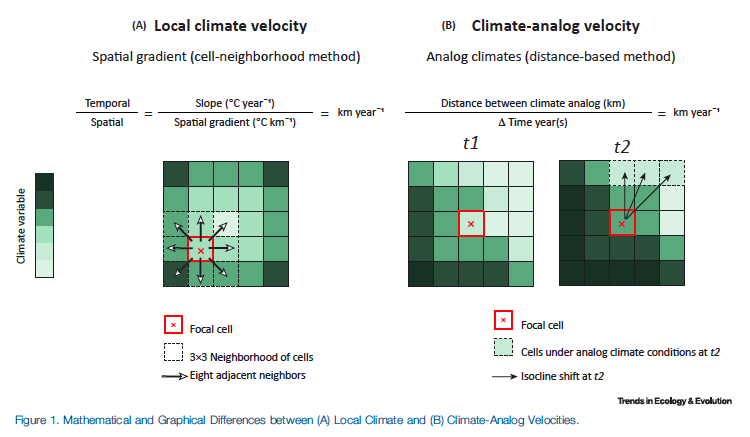
\includegraphics[width=1\linewidth]{images/VoCC_01}

To calculate \emph{climate velocity} the R package \texttt{VoCC} provides a comprehensive collection of functions that calculate climate velocity and related metrics from their initial formulation to the latest developments. See \href{https://besjournals.onlinelibrary.wiley.com/doi/full/10.1111/2041-210X.13295}{Garcia Molinos et al.~2019}.

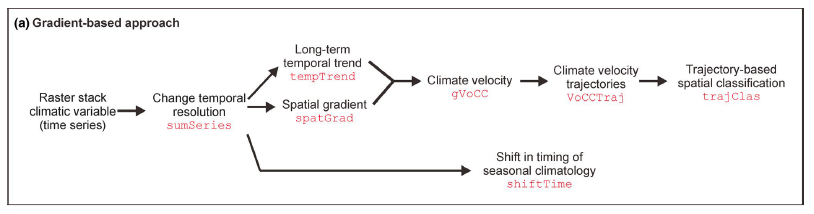
\includegraphics[width=1\linewidth]{images/VoCC_02}

\begin{Shaded}
\begin{Highlighting}[]
\CommentTok{# Load the monthly raster object}
\NormalTok{  rs <-}\StringTok{ }\NormalTok{raster}\OperatorTok{::}\KeywordTok{stack}\NormalTok{(}\StringTok{"data/ClimateModelsRasterMonthly/tos/ssp585/tos_Omon_GFDL-CM4_ssp585_2015-2100.grd"}\NormalTok{)}
\CommentTok{# Establish the time period of interest (if applicable)}
\NormalTok{  from =}\StringTok{ }\DecValTok{2020}
\NormalTok{  to =}\StringTok{ }\DecValTok{2100}
\CommentTok{# Define the time period to estimate climate velocity and subset the original raster}
\NormalTok{  names.yrs <-}\StringTok{ }\KeywordTok{paste}\NormalTok{(}\StringTok{"X"}\NormalTok{, }\KeywordTok{seq}\NormalTok{(}\KeywordTok{as.Date}\NormalTok{(}\KeywordTok{paste}\NormalTok{(from, }\StringTok{"1"}\NormalTok{, }\StringTok{"1"}\NormalTok{, }\DataTypeTok{sep =} \StringTok{"/"}\NormalTok{)), }\KeywordTok{as.Date}\NormalTok{(}\KeywordTok{paste}\NormalTok{(to, }\StringTok{"12"}\NormalTok{, }\StringTok{"1"}\NormalTok{, }\DataTypeTok{sep =} \StringTok{"/"}\NormalTok{)), }\DataTypeTok{by =} \StringTok{"month"}\NormalTok{), }\DataTypeTok{sep =} \StringTok{""}\NormalTok{) }\OperatorTok
\StringTok{    }\KeywordTok{str_replace_all}\NormalTok{(}\DataTypeTok{pattern =} \StringTok{"-"}\NormalTok{, }\DataTypeTok{replacement =} \StringTok{"."}\NormalTok{)}
\NormalTok{  rs <-}\StringTok{ }\NormalTok{raster}\OperatorTok{::}\KeywordTok{subset}\NormalTok{(rs, names.yrs)}
\CommentTok{# If Raster is monthly, get annual mean}
\NormalTok{  index <-}\StringTok{ }\KeywordTok{rep}\NormalTok{(}\DecValTok{1}\OperatorTok{:}\KeywordTok{nlayers}\NormalTok{(rs), }\DataTypeTok{each =} \DecValTok{12}\NormalTok{, }\DataTypeTok{length.out =} \KeywordTok{nlayers}\NormalTok{(rs))}
\NormalTok{  rs <-}\StringTok{ }\KeywordTok{stackApply}\NormalTok{(}\DataTypeTok{x =}\NormalTok{ rs, }\DataTypeTok{indices =}\NormalTok{ index, }\DataTypeTok{fun =}\NormalTok{ mean)}
  
\CommentTok{# Calculate VoCC}
  \CommentTok{# Temporal trend (slope)}
\NormalTok{    slp <-}\StringTok{ }\KeywordTok{tempTrend}\NormalTok{(rs, }\DataTypeTok{th =} \DecValTok{10}\NormalTok{)}
  \CommentTok{# Spatial gradient (gradient)}
\NormalTok{    grad <-}\StringTok{ }\KeywordTok{spatGrad}\NormalTok{(rs, }\DataTypeTok{th =} \FloatTok{0.0001}\NormalTok{, }\DataTypeTok{projected =} \OtherTok{FALSE}\NormalTok{)}
  \CommentTok{# VoCC local gradient}
\NormalTok{    vocc <-}\StringTok{ }\KeywordTok{gVoCC}\NormalTok{(slp, grad)}
\NormalTok{    vocc}\OperatorTok{$}\NormalTok{voccMag[] <-}\StringTok{ }\KeywordTok{ifelse}\NormalTok{(}\KeywordTok{is.infinite}\NormalTok{(vocc}\OperatorTok{$}\NormalTok{voccMag[]), }\OtherTok{NA}\NormalTok{, vocc}\OperatorTok{$}\NormalTok{voccMag[]) }\CommentTok{# replace inf with NAs}
\end{Highlighting}
\end{Shaded}

\hypertarget{relative-climate-exposure-rce}{%
\section{Relative Climate Exposure (RCE)}\label{relative-climate-exposure-rce}}

The RCE is a metric that we developed to obtain information about the amount of exposure to climate warming that local populations of a species would face relative to its experience of variation in seasonal temperatures \href{https://www.researchsquare.com/article/rs-421078/v1}{Brito-Morales et al.~2021}. RCE is calculated as the ratio of the slope of a linear regression of projected mean annual temperatures (°C yr-1) to the current mean seasonal temperature range (°C):

\begin{Shaded}
\begin{Highlighting}[]
\CommentTok{# The current seasonal variation (could be any range)}
\NormalTok{  from =}\StringTok{ }\DecValTok{2016}
\NormalTok{  to =}\StringTok{ }\DecValTok{2021}
\CommentTok{# Getting the years/month to calculate de RCE index}
\NormalTok{  names.yrs <-}\StringTok{ }\KeywordTok{paste}\NormalTok{(}\StringTok{"X"}\NormalTok{, }\KeywordTok{seq}\NormalTok{(}\KeywordTok{as.Date}\NormalTok{(}\KeywordTok{paste}\NormalTok{(from, }\StringTok{"1"}\NormalTok{, }\StringTok{"1"}\NormalTok{, }\DataTypeTok{sep =} \StringTok{"/"}\NormalTok{)), }
                              \KeywordTok{as.Date}\NormalTok{(}\KeywordTok{paste}\NormalTok{(to, }\StringTok{"12"}\NormalTok{, }\StringTok{"1"}\NormalTok{, }\DataTypeTok{sep =} \StringTok{"/"}\NormalTok{)), }\DataTypeTok{by =} \StringTok{"month"}\NormalTok{), }
                     \DataTypeTok{sep =} \StringTok{""}\NormalTok{) }\OperatorTok
\StringTok{    }\KeywordTok{str_replace_all}\NormalTok{(}\DataTypeTok{pattern =} \StringTok{"-"}\NormalTok{, }\DataTypeTok{replacement =} \StringTok{"."}\NormalTok{)}
\CommentTok{# Read and subset the data}
\NormalTok{  rs <-}\StringTok{ }\KeywordTok{readAll}\NormalTok{(raster}\OperatorTok{::}\KeywordTok{stack}\NormalTok{(}\StringTok{"data/ClimateModelsRasterMonthly/tos/ssp585/tos_Omon_GFDL-CM4_ssp585_2015-2100.grd"}\NormalTok{)) }\OperatorTok\StringTok{ }
\StringTok{    }\KeywordTok{subset}\NormalTok{(names.yrs)}
\CommentTok{# Annual min and max to estimate the rage to get the RCE}
\NormalTok{  index <-}\StringTok{ }\KeywordTok{rep}\NormalTok{(}\DecValTok{1}\OperatorTok{:}\KeywordTok{nlayers}\NormalTok{(rs), }\DataTypeTok{each =} \DecValTok{12}\NormalTok{, }\DataTypeTok{length.out =} \KeywordTok{nlayers}\NormalTok{(rs))}
\NormalTok{  rs_min <-}\StringTok{ }\KeywordTok{stackApply}\NormalTok{(}\DataTypeTok{x =}\NormalTok{ rs, }\DataTypeTok{indices =}\NormalTok{ index, }\DataTypeTok{fun =}\NormalTok{ min)}
\NormalTok{  rs_max <-}\StringTok{ }\KeywordTok{stackApply}\NormalTok{(}\DataTypeTok{x =}\NormalTok{ rs, }\DataTypeTok{indices =}\NormalTok{ index, }\DataTypeTok{fun =}\NormalTok{ max)}
\CommentTok{# Range among the period selected}
\NormalTok{  rs_range <-}\StringTok{ }\NormalTok{rs_max }\OperatorTok{-}\StringTok{ }\NormalTok{rs_min}
\NormalTok{  rs_range_mean <-}\StringTok{ }\KeywordTok{stackApply}\NormalTok{(}\DataTypeTok{x =}\NormalTok{ rs_range, }\DataTypeTok{indices =} \KeywordTok{nlayers}\NormalTok{(rs_range), }\DataTypeTok{fun =}\NormalTok{ mean)}
  
\CommentTok{# Get the slope}
\NormalTok{  from =}\StringTok{ }\DecValTok{2020}
\NormalTok{  to =}\StringTok{ }\DecValTok{2100}
\NormalTok{  names.yrs <-}\StringTok{ }\KeywordTok{paste}\NormalTok{(}\StringTok{"X"}\NormalTok{, }\KeywordTok{seq}\NormalTok{(}\KeywordTok{as.Date}\NormalTok{(}\KeywordTok{paste}\NormalTok{(from, }\StringTok{"1"}\NormalTok{, }\StringTok{"1"}\NormalTok{, }\DataTypeTok{sep =} \StringTok{"/"}\NormalTok{)), }\KeywordTok{as.Date}\NormalTok{(}\KeywordTok{paste}\NormalTok{(to, }\StringTok{"12"}\NormalTok{, }\StringTok{"1"}\NormalTok{, }\DataTypeTok{sep =} \StringTok{"/"}\NormalTok{)), }\DataTypeTok{by =} \StringTok{"month"}\NormalTok{), }\DataTypeTok{sep =} \StringTok{""}\NormalTok{) }\OperatorTok
\StringTok{    }\KeywordTok{str_replace_all}\NormalTok{(}\DataTypeTok{pattern =} \StringTok{"-"}\NormalTok{, }\DataTypeTok{replacement =} \StringTok{"."}\NormalTok{)}
\NormalTok{  rs <-}\StringTok{ }\NormalTok{raster}\OperatorTok{::}\KeywordTok{stack}\NormalTok{(}\StringTok{"data/ClimateModelsRasterMonthly/tos/ssp585/tos_Omon_GFDL-CM4_ssp585_2015-2100.grd"}\NormalTok{) }\OperatorTok\StringTok{ }
\StringTok{    }\KeywordTok{subset}\NormalTok{(names.yrs)}
\NormalTok{  index <-}\StringTok{ }\KeywordTok{rep}\NormalTok{(}\DecValTok{1}\OperatorTok{:}\KeywordTok{nlayers}\NormalTok{(rs), }\DataTypeTok{each =} \DecValTok{12}\NormalTok{, }\DataTypeTok{length.out =} \KeywordTok{nlayers}\NormalTok{(rs))}
\NormalTok{  rs <-}\StringTok{ }\KeywordTok{stackApply}\NormalTok{(}\DataTypeTok{x =}\NormalTok{ rs, }\DataTypeTok{indices =}\NormalTok{ index, }\DataTypeTok{fun =}\NormalTok{ mean)}
\NormalTok{  slp <-}\StringTok{ }\NormalTok{((}\KeywordTok{tempTrend}\NormalTok{(rs, }\DataTypeTok{th =} \DecValTok{10}\NormalTok{))}\OperatorTok{*}\DecValTok{10}\NormalTok{)}\OperatorTok{*}\DecValTok{8} \CommentTok{# x10 decadal and x8 for decades (2020-2100)}

\CommentTok{# Calculate the RCE}
\NormalTok{  RCE <-}\StringTok{ }\KeywordTok{abs}\NormalTok{(slp}\OperatorTok{/}\NormalTok{rs1_range_mean)}
\end{Highlighting}
\end{Shaded}

\hypertarget{raster-objects-and-spatial-object}{%
\chapter{Raster objects and Spatial object}\label{raster-objects-and-spatial-object}}

\hypertarget{introduction-2}{%
\section{Introduction}\label{introduction-2}}

The aim here is to provide a worked example of how intersect rasters with spatial polygon objects using the \emph{sf R} and \emph{exactextractr R} packages.

This example used two objects.

\begin{itemize}
\tightlist
\item
  \textbf{spatial polygon object}: located at \texttt{data/PlanningUnits/PUs\_WeddellSea\_100km2.shp}. This object contains hexagonal polygons of equal area. It has two columns: integer unique identifiers (``id''), geometry information (``geometry'')\\
\item
  \textbf{raster object}: located at \texttt{data/VoCC/tos/voccMag\_tos\_GFDL-CM4\_ssp585\_2015-2100.grd\_2050-2100\_.tif}. This object is a raster \emph{.tif} object of climate-velocity estimates in the southern ocean.
\end{itemize}

The objective here is to assign to eash hexagon in the \emph{spatial polygon object} a climate velocity value

\hypertarget{data-import-2}{%
\section{Data import}\label{data-import-2}}

First, load the required packages and the data.

\begin{Shaded}
\begin{Highlighting}[]
\CommentTok{# load packages}
  \KeywordTok{library}\NormalTok{(raster)}
  \KeywordTok{library}\NormalTok{(sf)}
  \KeywordTok{library}\NormalTok{(dplyr)}
  \KeywordTok{library}\NormalTok{(exactextractr)}
  \KeywordTok{library}\NormalTok{(stringr)}
  \KeywordTok{library}\NormalTok{(nngeo)}
\end{Highlighting}
\end{Shaded}

\hypertarget{function-to-replace-nas-with-nearest-neighbor}{%
\section{Function to replace NAs with nearest neighbor}\label{function-to-replace-nas-with-nearest-neighbor}}

This functions helps to replace NAs with nearest neighbor interpolation method.

\begin{Shaded}
\begin{Highlighting}[]
\CommentTok{# Function to replace NAs with nearest neighbor. Function wrtitten by Jason Everett}
\NormalTok{  fCheckNAs <-}\StringTok{ }\ControlFlowTok{function}\NormalTok{(df, vari) \{}
    \ControlFlowTok{if}\NormalTok{ (}\KeywordTok{sum}\NormalTok{(}\KeywordTok{is.na}\NormalTok{(}\KeywordTok{pull}\NormalTok{(df, }\OperatorTok{!!}\KeywordTok{sym}\NormalTok{(vari))))}\OperatorTok{>}\DecValTok{0}\NormalTok{)\{ }\CommentTok{# Check if there are NAs}
\NormalTok{      gp <-}\StringTok{ }\NormalTok{df }\OperatorTok
\StringTok{        }\KeywordTok{mutate}\NormalTok{(}\DataTypeTok{isna =} \KeywordTok{is.finite}\NormalTok{(}\OperatorTok{!!}\KeywordTok{sym}\NormalTok{(vari))) }\OperatorTok
\StringTok{        }\KeywordTok{group_by}\NormalTok{(isna) }\OperatorTok
\StringTok{        }\KeywordTok{group_split}\NormalTok{()}
      
\NormalTok{      out_na <-}\StringTok{ }\NormalTok{gp[[}\DecValTok{1}\NormalTok{]] }\CommentTok{# DF with NAs}
\NormalTok{      out_finite <-}\StringTok{ }\NormalTok{gp[[}\DecValTok{2}\NormalTok{]] }\CommentTok{# DF without NAs}
      
\NormalTok{      d <-}\StringTok{ }\KeywordTok{st_nn}\NormalTok{(out_na, out_finite) }\OperatorTok\StringTok{ }\CommentTok{# Get nearest neighbour}
\StringTok{        }\KeywordTok{unlist}\NormalTok{()}
\NormalTok{      out_na <-}\StringTok{ }\NormalTok{out_na }\OperatorTok
\StringTok{        }\KeywordTok{mutate}\NormalTok{(}\OperatorTok{!!}\KeywordTok{sym}\NormalTok{(vari) }\OperatorTok{:}\ErrorTok{=}\StringTok{ }\KeywordTok{pull}\NormalTok{(out_finite, }\OperatorTok{!!}\KeywordTok{sym}\NormalTok{(vari))[d])}
\NormalTok{      df <-}\StringTok{ }\KeywordTok{rbind}\NormalTok{(out_finite, out_na)}
\NormalTok{    \}}
    \KeywordTok{return}\NormalTok{(df)}
\NormalTok{  \}}
\end{Highlighting}
\end{Shaded}

\hypertarget{raster-by-spatial-polygon-object}{%
\section{Raster by spatial polygon object}\label{raster-by-spatial-polygon-object}}

The aim here is to provide an example of how integrate raster in an sf polygon spatial object

\begin{Shaded}
\begin{Highlighting}[]
\CommentTok{# Reading the spatial polygon object}
\NormalTok{  pu_region <-}\StringTok{ }\KeywordTok{st_read}\NormalTok{(}\StringTok{"data/PlanningUnits/PUs_WeddellSea_100km2.shp"}\NormalTok{)}
  \KeywordTok{st_crs}\NormalTok{(pu_region) <-}\StringTok{ "+proj=laea +lat_0=-90 +lon_0=0 +x_0=0 +y_0=0 +datum=WGS84 +units=m +no_defs"}
  
\CommentTok{# Reading the raster object}
\NormalTok{  vocc_file <-}\StringTok{ }\NormalTok{raster}\OperatorTok{::}\KeywordTok{raster}\NormalTok{(}\StringTok{"data/VoCC/tos/voccMag_tos_GFDL-CM4_ssp585_2015-2100.grd_2050-2100_.tif"}\NormalTok{)}
  \KeywordTok{crs}\NormalTok{(vocc_file) <-}\StringTok{ }\KeywordTok{CRS}\NormalTok{(}\StringTok{"+proj=longlat +datum=WGS84 +ellps=WGS84 +towgs84=0,0,0"}\NormalTok{)}
\NormalTok{  weight_rs_vocc <-}\StringTok{ }\NormalTok{raster}\OperatorTok{::}\KeywordTok{area}\NormalTok{(vocc_file)}
\NormalTok{  vocc_file <-}\StringTok{ }\KeywordTok{projectRaster}\NormalTok{(vocc_file, }\DataTypeTok{crs =} \KeywordTok{CRS}\NormalTok{(}\StringTok{"+proj=laea +lat_0=-90 +lon_0=0 +x_0=0 +y_0=0 +datum=WGS84 +units=m +no_defs"}\NormalTok{), }
                             \DataTypeTok{method =} \StringTok{"ngb"}\NormalTok{, }\DataTypeTok{over =} \OtherTok{FALSE}\NormalTok{)}
\NormalTok{  weight_vocc <-}\StringTok{ }\KeywordTok{projectRaster}\NormalTok{(weight_rs_vocc, }\DataTypeTok{crs =} \KeywordTok{CRS}\NormalTok{(}\StringTok{"+proj=laea +lat_0=-90 +lon_0=0 +x_0=0 +y_0=0 +datum=WGS84 +units=m +no_defs"}\NormalTok{), }
                               \DataTypeTok{method =} \StringTok{"ngb"}\NormalTok{, }\DataTypeTok{over =} \OtherTok{FALSE}\NormalTok{)}
  \KeywordTok{names}\NormalTok{(vocc_file) <-}\StringTok{ "layer"}
  
\CommentTok{# Getting the value by planning unit}
\NormalTok{  vocc_bypu <-}\StringTok{ }\KeywordTok{exact_extract}\NormalTok{(vocc_file, pu_region, }\StringTok{"weighted_mean"}\NormalTok{, }\DataTypeTok{weights =}\NormalTok{ weight_vocc)}
\NormalTok{  vocc_shp <-}\StringTok{ }\NormalTok{pu_region }\OperatorTok
\StringTok{    }\NormalTok{dplyr}\OperatorTok{::}\KeywordTok{mutate}\NormalTok{(}\DataTypeTok{vocc =}\NormalTok{ vocc_bypu) }\OperatorTok
\StringTok{    }\NormalTok{dplyr}\OperatorTok{::}\KeywordTok{relocate}\NormalTok{(cellID, vocc)}
\CommentTok{# Replace NAs with nearest neighbor}
\NormalTok{  vocc_sfInt <-}\StringTok{ }\KeywordTok{fCheckNAs}\NormalTok{(}\DataTypeTok{df =}\NormalTok{ vocc_shp, }\DataTypeTok{vari =} \KeywordTok{names}\NormalTok{(vocc_shp)[}\DecValTok{2}\NormalTok{]) }\OperatorTok
\StringTok{  }\NormalTok{dplyr}\OperatorTok{::}\KeywordTok{select}\NormalTok{(}\OperatorTok{-}\NormalTok{isna)}
\end{Highlighting}
\end{Shaded}

\hypertarget{spatial-polygon-object-by-region-of-interest}{%
\section{Spatial polygon object by region of interest}\label{spatial-polygon-object-by-region-of-interest}}

The aim here is to provide a simple script to assign a Longhurst province identifier per planning unit

\begin{Shaded}
\begin{Highlighting}[]
\CommentTok{# Reading the spatial polygon object}
\NormalTok{  pu_region <-}\StringTok{ }\KeywordTok{st_read}\NormalTok{(}\StringTok{"data/PlanningUnits/PUs_WeddellSea_100km2.shp"}\NormalTok{) }\OperatorTok\StringTok{ }
\StringTok{    }\KeywordTok{st_transform}\NormalTok{(}\DataTypeTok{crs =} \KeywordTok{CRS}\NormalTok{(}\StringTok{"+proj=laea +lat_0=-90 +lon_0=0 +x_0=0 +y_0=0 +datum=WGS84 +units=m +no_defs"}\NormalTok{))}
\CommentTok{# Reading Longhurst Provinces Shapefile}
\NormalTok{  bioprovince <-}\StringTok{ }\KeywordTok{st_read}\NormalTok{(}\StringTok{"data/Boundaries/LonghurstProvinces/Longhurst_world_v4_2010.shp"}\NormalTok{) }\OperatorTok\StringTok{ }
\StringTok{    }\KeywordTok{st_transform}\NormalTok{(}\DataTypeTok{crs =} \KeywordTok{CRS}\NormalTok{(}\StringTok{"+proj=laea +lat_0=-90 +lon_0=0 +x_0=0 +y_0=0 +datum=WGS84 +units=m +no_defs"}\NormalTok{)) }\OperatorTok\StringTok{ }
\StringTok{    }\KeywordTok{st_make_valid}\NormalTok{()}
\CommentTok{# Get the Longhurst Provinces per Planning unit}
\NormalTok{  nr <-}\StringTok{ }\KeywordTok{st_nearest_feature}\NormalTok{(pu_region, bioprovince)}
\NormalTok{  pu_region <-}\StringTok{ }\NormalTok{pu_region }\OperatorTok\StringTok{ }
\StringTok{    }\NormalTok{dplyr}\OperatorTok{::}\KeywordTok{mutate}\NormalTok{(}\DataTypeTok{province =} \KeywordTok{paste}\NormalTok{(}\KeywordTok{as.vector}\NormalTok{(bioprovince}\OperatorTok{$}\NormalTok{ProvCode[nr]), prov_name, }\DataTypeTok{sep =} \StringTok{"_"}\NormalTok{)) }\OperatorTok\StringTok{ }
\StringTok{    }\NormalTok{dplyr}\OperatorTok{::}\KeywordTok{arrange}\NormalTok{(layer)}
\end{Highlighting}
\end{Shaded}

\bibliography{book.bib,packages.bib}

\end{document}
